% !TEX program = pdflatex
\documentclass[11pt,a4paper]{article}
\usepackage[T1]{fontenc}
\usepackage[utf8]{inputenc}
\usepackage{lmodern}
\usepackage{textcomp}
\usepackage[english]{babel}
\usepackage{amsmath,amssymb}
\usepackage{graphicx}
\usepackage[a4paper,margin=2.4cm]{geometry}
\usepackage{array}
\usepackage{xcolor}
\usepackage{hyperref}
\usepackage{float}

% --- minimal stand-ins for siunitx and booktabs (not in this distribution) ---
\providecommand{\toprule}{\hline}
\providecommand{\midrule}{\hline}
\providecommand{\bottomrule}{\hline}
\providecommand{\micro}{\textmu}
\providecommand{\degreeCelsius}{\textcelsius}
\providecommand{\SI}[2]{#1\,\text{#2}}
\providecommand{\num}[1]{#1}

\hypersetup{colorlinks=true,linkcolor=blue!55!black,citecolor=blue!55!black,
  urlcolor=blue!55!black,pdftitle={Photonic Engine V6 - Optically Guided Rotor},
  pdfauthor={Francesco Bulla}}

\setlength{\parskip}{0.35em}
\setlength{\parindent}{1.2em}

\title{\bfseries The optically guided rotor\\[0.3em]
\large Torque limits, dissipation and stability in the Photonic Engine of the Vacuum\\
\large Revision V6}
\author{Francesco Bulla\\ \small Catania, Italy}
\date{28 October 2026 \quad \small version 6.1}

\begin{document}
\maketitle

\begin{abstract}
\noindent
V6 does not add parts to V5: it removes ambiguities and puts the model in a position
to be refuted. The work rests on three choices. The first is a single model,
declared as a \emph{limit}: $\tau=(\ell+s)P_{\rm abs}/\omega_{\rm ott}$ and
$F=I\sigma_{\rm pr}/c$, two distinct channels rather than two ways of saying the same
thing. The second is a drag coefficient declared as an \emph{interval}, bounded by
the minimum-dissipation theorem and by slender-body theory. The third is that every
number in the text comes from a data file generated by the enclosed code.

This 6.1 revision corrects five material errors of 6.0. The wire radii are those of
the V5 scene (3.2 / 7.5 / 4.5 nm, i.e. diameters of 6.4 / 15 / 9 nm) and not
1.25 nm: since in the Rayleigh regime $\sigma\propto a^2$, the cross-sections grow by
47\,\% ($\sigma_{\rm pr}=1.065\times10^{-14}$\,m$^2$ against $7.259\times10^{-15}$)
and the mass goes from $2.78$ to $8.21\times10^{-18}$\,kg. The radiating area is the
real metal surface ($2.69\times10^{-13}$\,m$^2$), not the spherical envelope, and in
vacuum the rotor already melts at \SI{1}{\micro W}: \SI{2250}{K} with
$\epsilon=0.03$, \SI{1505}{K} with $\epsilon=0.15$, against a melting point of
\SI{1358}{K}. The melting threshold is \SI{0.13}{}--\SI{0.66}{\micro W} of incident
power and the adiabatic time is \SI{0.28}{ms}. The equal-mass comparison is recast as
a conditional statement: for the drag the result is robust (three decades of
variation), for the torque it depends on the shape-dependent cross-section, which a
DDA calculation still has to supply. The comparison with silica rotors at 1--6\,GHz
becomes a consistency check on the mechanical scale: the observed $(f,r)$ pairs imply
an effective strength between $0.22$ and $7.8$\,GPa, which is the order of magnitude
of nanoscale silica, and nothing more. Finally, OAM is not a multiplier: including
the mode overlap, the net gain at $\ell=5$ is $1.05$, not $6$.

The result that survives every correction is that, at \SI{1}{\micro W} in water, the
optical torque gives $Pe_r=7.7\times10^{-4}$, and the frame drag exceeds that of the
bare core by a factor 209: the rotor is not oriented, and geometry does not save it.
\end{abstract}

\vspace{0.3em}
\noindent\rule{\textwidth}{0.4pt}
\section*{Eight results}
\addcontentsline{toc}{section}{Eight results}
\begin{enumerate}\itemsep2pt
\item \textbf{Wire radii corrected.} 3.2 / 7.5 / 4.5 nm, not 1.25 nm: cross-sections
grow by 47\,\%, mass from $5.73$ to $8.21\times10^{-18}$\,kg, moment of inertia from
$3.09\times10^{-32}$ to $4.62\times10^{-31}$\,kg\,m$^2$.
\item \textbf{Torque.} $\tau=3.31\times10^{-24}$\,N\,m (+27\,\% over V5): it uses
$P_{\rm abs}=11.70$\,nW, not $P_{\rm int}=13.56$\,nW.
\item \textbf{Drag.} $\beta\in[4.04,\,6.48]\times10^{-22}$\,N\,m\,s against
$2.89\times10^{-23}$ in V5, which sits at 7\,\% of the lower bound.
\item \textbf{Figure of merit.} $Pe_r=7.72\times10^{-4}$: optical rotation is three
orders of magnitude below Brownian noise.
\item \textbf{Thermal.} In vacuum, at \SI{1}{\micro W}: \SI{2250}{K} or \SI{1505}{K}
depending on emissivity, i.e. the rotor melts. Threshold:
\SI{0.13}{}--\SI{0.66}{\micro W}.
\item \textbf{Baseline.} At equal mass the lattice has the highest drag of all
geometries ($\beta$ 6 to 98 times) and the lowest torque (0.44 of the compact sphere).
\item \textbf{External check.} Observations at 1--6\,GHz imply
$\sigma_y=0.22$--$7.8$\,GPa: mechanical-scale consistency, not optical validation.
\item \textbf{OAM.} Net gain $1.05$ at $\ell=5$: the mode overlap cancels the $\ell$
factor.
\end{enumerate}
\noindent\rule{\textwidth}{0.4pt}

\begin{figure}[H]
\centering
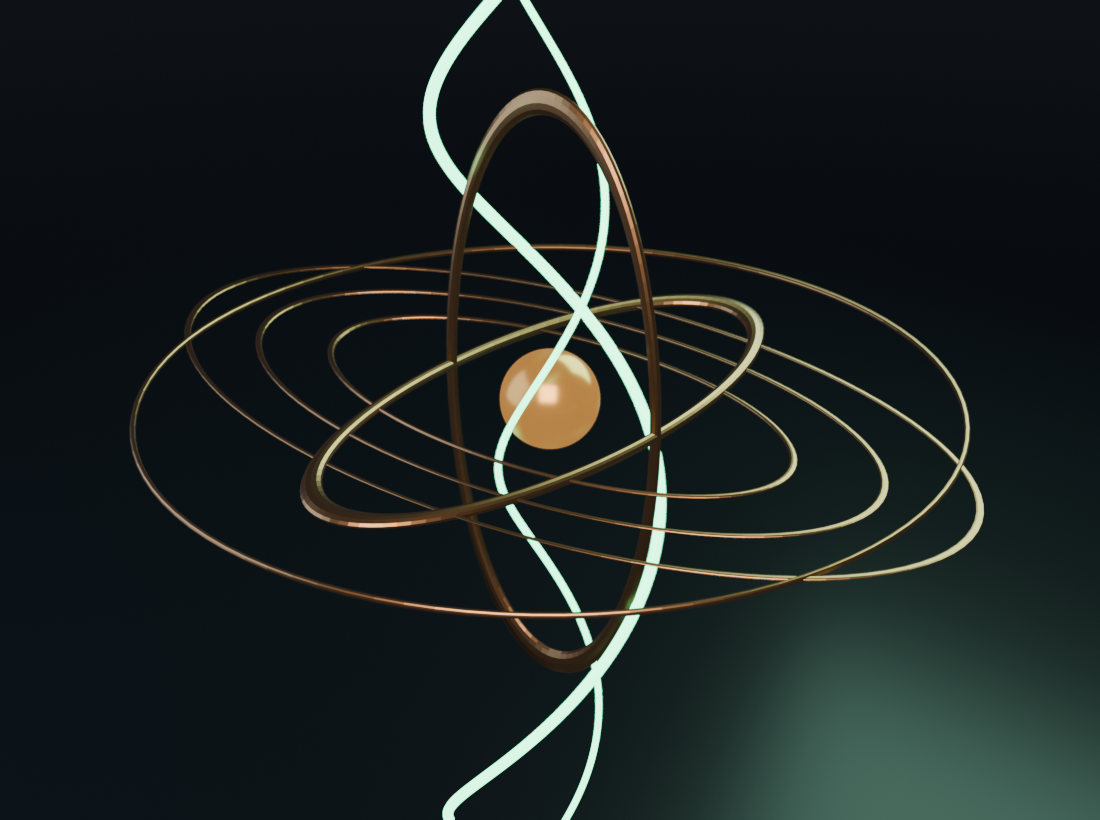
\includegraphics[width=0.86\textwidth]{../blender/rotore_hero.png}
\caption{The optically guided rotor: wire frame, copper core and a beam carrying
orbital angular momentum. The Blender scene is built with the proportions of the
model (1 unit $=$ 100\,nm) and the wire radii of the V5 scene; the beam is drawn as a
helix, not a cylinder, because what matters is not its shape but the angular
momentum it carries.}
\label{fig:hero}
\end{figure}

\tableofcontents
\newpage

%=====================================================================
\section{Thesis and criteria}
%=====================================================================

V5 closed with an honest sentence: the model does not claim experimental validation.
V6 starts there and changes the criterion of success. It does not ask whether the
architecture is plausible, but whether its quantities are compatible with independent
measurements, and under which conditions they are not.

The title changed accordingly. No longer \emph{engine}, with the promise of thrust the
word carries, but \emph{optically guided rotor}: a body held and spun by a beam, whose
torque, dissipation and thermal stability are studied.\footnote{Note on the figures:
the twelve figures are shared with the Italian edition and keep Italian axis labels;
captions are translated.} The difference is not nominal.
An engine is judged by useful work; a guided rotor is judged by two numbers, both
measurable:
\begin{equation}
\boxed{\;\eta_{\rm int}=\frac{\sigma_{\rm pr}}{A_{\rm beam}},
\qquad
Pe_r=\frac{\tau}{k_BT}=\frac{\omega_{\rm ss}}{D_r}\;}
\label{eq:merito}
\end{equation}
$\eta_{\rm int}$ says how much of the available light actually touches the structure;
$Pe_r$ says whether the optical torque survives orientational noise. The second is the
number that matters: below $Pe_r=1$ the rotor is not oriented, it is merely warmer.

The four criteria by which this revision should be judged are those stated at the
outset, and I adopt them as a commitment: how much angular momentum light actually
transfers; how much of it survives dissipation and thermal limits; whether the
Spin/Counter-spin geometry offers an advantage at equal mass; whether the predictions
are compatible with independent results.

The answers of V6 are, in order: little (the limit
$(\ell+s)P_{\rm abs}/\omega_{\rm ott}$, with $P_{\rm abs}$ equal to 86\,\% of
$P_{\rm int}$); almost nothing (the torque is $10^{-4}\,k_BT$, and in vacuum melting
comes before spin-up); no (the frame is a brake); yes, but only on the mechanical
scale. None of the four is a failure of the work: they are the reason the work makes
sense.

\subsection{What changes with respect to V5}

\begin{table}[H]
\centering\small
\caption{Quantities declared by V5 and values computed by V6. The first two rows show
that the V5 error was not in the model but in the geometry: with the wrong wire radii
the cross-sections are underestimated by 47\,\%.}
\label{tab:confronto}
\begin{tabular}{lrrr}
\toprule
Quantity & V5 & V6 & cause \\
\midrule
$\sigma_{\rm pr}$ & $7.259\times10^{-15}$\,m$^2$ & $1.065\times10^{-14}$\,m$^2$ & wire radii \\
$F$ & $3.083\times10^{-17}$\,N & $4.522\times10^{-17}$\,N & wire radii \\
$\tau$ & $2.610\times10^{-24}$\,N\,m & $3.305\times10^{-24}$\,N\,m & $P_{\rm abs}\neq P_{\rm int}$ \\
$\beta$ & $2.89\times10^{-23}$\,N\,m\,s & $4.04$--$6.48\times10^{-22}$ & physical interval \\
$\omega_{\rm ss}$ & $1.14\times10^{-1}$\,rad/s & $5.1$--$8.2\times10^{-3}$\,rad/s & consequence of $\beta$ \\
$Pe_r$ & $6.10\times10^{-4}$ & $7.72\times10^{-4}$ & identity $\tau/k_BT$ \\
\bottomrule
\end{tabular}
\end{table}

%=====================================================================
\section{Closing the residuals}
%=====================================================================

None of the inconsistencies flagged in the review requires a measurement: they close
with exact arithmetic and the right geometry. Table~\ref{tab:residui} lists them,
Figure~\ref{fig:residui} shows the two most important.

\begin{table}[H]
\centering\small
\caption{Residuals and their closure. V6 values are produced by
\texttt{v6\_studi.py}.}
\label{tab:residui}
\begin{tabular}{p{2.9cm}p{3.0cm}p{3.0cm}p{5.5cm}}
\hline
Quantity & V5 & V6 & note \\
\hline
Ratio $\omega_2/\omega_1$ & 0.119667646 & $45/376=0.119680851$ & the V5 value is not
$8.3565$ (i.e. $0.11966732$) but $1/8.35648$: it cannot be reconstructed from the
declared data \\
$I_2/I_1$ & 8.353816 & $376/45=8.355556$ & offset $-2.1\times10^{-4}$; closure
requires the mass of App.~A \\
$r_{\rm eff}$ & 239.93 nm & 60.26 / 259.34 nm & material volume / hydrodynamic radius:
two different quantities \\
Mass & $5.73\times10^{-18}$ kg & $8.21\times10^{-18}$ kg & V5 counted the wires only; V6
adds the core (29\,\% of the total) \\
Force $F$ & $3.08\times10^{-17}$ N & $4.52\times10^{-17}$ N & $+47$\,\%: wire radii
3.2 / 7.5 / 4.5 nm, not 1.25 nm \\
Torque $\tau$ & $2.61\times10^{-24}$ N\,m & $3.31\times10^{-24}$ N\,m & $+27$\,\%:
$P_{\rm abs}$ and not $P_{\rm int}$, with the corrected cross-sections \\
$Pe_r$ & $6.10\times10^{-4}$ & $7.72\times10^{-4}$ & identity $\tau/k_BT$; V5 also
quoted $8.8\times10^{-3}$ with a different $\beta$ \\
\hline
\end{tabular}
\end{table}

\subsection{The number 0.119667646 is not a rounding of 45/376}

V5 reported, in a caption, an offset of $-1.32\times10^{-5}$ between the kinematic and
the inertial ratio. The number cannot be reconstructed. The printed value,
$0.119667646$, equals $1/8.35648$; $1/8.3565$ equals $0.11966732$; $45/376$ equals
$0.119680851$. These are three different numbers, and none follows from the others.
The ratio $I_2/I_1$ of the V4 data is $8.353816$, which against the target $8.355556$
gives $-2.1\times10^{-4}$: this is the real residual, and it is a property of the
geometry, not a rounding slip. V6 publishes $I_1$ computed from the geometry
($4.62\times10^{-31}$\,kg\,m$^2$) and treats $I_2$ as the unknown of the constraint,
not as data.

\subsection{The equivalent radius is not a radius}

V5 defined $r_{\rm eff}=239.93$\,nm as ``the radius of the sphere with the same volume
as the model''. Three volumes are in play and the sentence conflates two:
$r_{\rm volume}=60.3$\,nm (sphere with the \emph{material} volume,
$9.16\times10^{5}$\,nm$^3$), $r_{\rm envelope}=423.5$\,nm (the cylindrical envelope,
essentially empty) and $r_{\rm hydro}=259.3$\,nm (the sphere with the same $\beta$).
Only the last is useful, because $D$ and $D_r$ follow from $\beta$, not from the
volume. The \SI{239.93}{nm} of V5 is close to $r_{\rm hydro}$, so the number was
defensible; its justification was not. In V6 the radius appears once, where it is
needed, and it is called $\beta$.

\subsection{Mass: V5 counted the wires only}

The V5 mass, $5.734\times10^{-18}$\,kg, corresponds exactly to the wires at the scene
radii ($0.640$\,u.a.$^3\times8960$\,kg/m$^3$) and does not include the core. V6 uses
$8.211\times10^{-18}$\,kg: wires $5.81\times10^{-18}$ plus core $2.40\times10^{-18}$.
The thrust-to-weight ratio at $1\,g$ goes from $0.56$ to $0.63$ including buoyancy in
water; in orbit it is undefined, and that is the only sensible statement about a
``thrust'' of $4.5\times10^{-17}$\,N.

\subsection{Pulsed operation is not a property of the rotor}

The mechanical time constant is $I/\beta=1.14\times10^{-9}$\,s, i.e. a cutoff of
\SI{140}{MHz}. Any pulse longer than a nanosecond is quasi-static: pulsing changes
neither $\omega_{\rm ss}$ nor $Pe_r$, only the mean temperature. The duty cycle that
avoids melting in vacuum is $0.13$ at \SI{1}{\micro W} peak and $1.3\times10^{-5}$ at
\SI{10}{mW}. The natural signal period remains $\pi$, not $4\pi$: the two-lobe torque
repeats after 180$^\circ$, and the $SU(2)$ covering belongs in the appendix.

\begin{figure}[H]
\centering
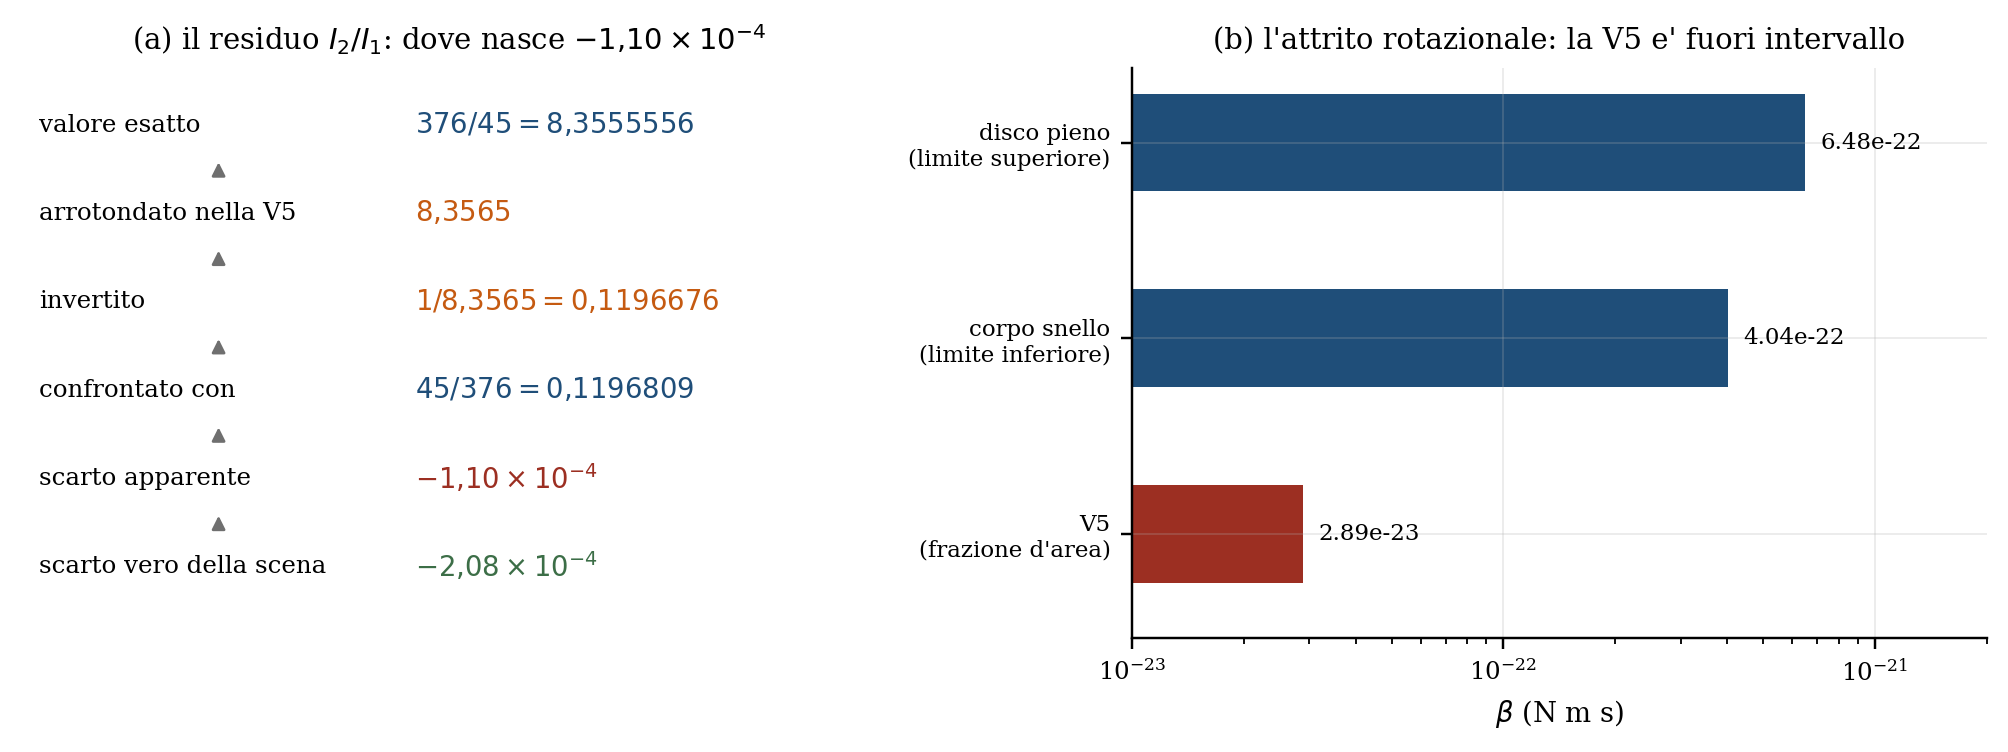
\includegraphics[width=\textwidth]{../figure/fig10_residui.png}
\caption{\textbf{(a)} The chain of values that produces the V5 number: none of the
three coincides, and the real residual is the scene one ($-2.1\times10^{-4}$).
\textbf{(b)} Rotational drag: the V5 estimate (wetted-area fraction) lies below the
lower bound from slender-body theory, hence outside the physically allowed interval.}
\label{fig:residui}
\end{figure}

%=====================================================================
\section{The single model}
%=====================================================================

V5 used three definitions of torque in different places. V6 uses one, and declares it
for what it is: a limit.
\begin{equation}
\tau=(\ell+s)\,\frac{P_{\rm abs}}{\omega_{\rm ott}},
\qquad
F=\frac{I\,\sigma_{\rm pr}}{c},
\qquad
\omega_{\rm ott}=\frac{2\pi c}{\lambda},
\label{eq:modello}
\end{equation}
with $\ell$ the orbital angular momentum per photon, $s=\pm1$ the spin one,
$I=P/A_{\rm beam}$ and $\sigma_{\rm pr}=\sigma_{\rm ext}-g\,\sigma_{\rm sca}$.

\subsection{Why they are two limits}

The first equation says: every absorbed photon delivers all its angular momentum
$(\ell+s)\hbar$. That is true only if absorption is complete and if angular momentum
is not handed back to the field; for the \SI{40}{nm} core absorption is 79\,\% of
extinction, so the limit is reasonable but not exact. The second says: every
intercepted photon delivers all its axial momentum, and fails when scattering is
forward ($g\to1$).

The two equations must not be added: they are distinct channels, and the second
produces no torque if the beam is symmetric. The methodological point is that
\emph{neither contains the radius}. In the single model the torque depends on absorbed
power and on angular momentum per photon, not on the size of the rotor. Geometry
enters $\beta$ and $I$, i.e. the response, not the drive.

\subsection{The identity V5 violated}

From \eqref{eq:modello} and $D_r=k_BT/\beta$ it follows that
\begin{equation}
Pe_r=\frac{\omega_{\rm ss}}{D_r}=\frac{\tau/\beta}{k_BT/\beta}=\frac{\tau}{k_BT},
\label{eq:identita}
\end{equation}
independently of $\beta$. V5 quoted two values for the same quantity,
$6.1\times10^{-4}$ and $8.8\times10^{-3}$, precisely because the second calculation
used the frame $\beta$ and the first the diffusion of the equivalent sphere. Identity
\eqref{eq:identita} is a consistency test the code runs at every execution.

Since $P_{\rm abs}=\eta_{\rm abs}P$ and $P/\omega_{\rm ott}=\dot N\hbar$,
\eqref{eq:identita} reads $Pe_r=(\ell+s)\dot N_{\rm abs}\hbar/k_BT$. The threshold
$Pe_r=1$ is a condition on the \emph{rate} of angular momentum: it requires
$k_BT/\hbar=4.1\times10^{13}$ quanta per second, i.e. \SI{15}{\micro W} of absorbed
power with $\ell+s=1$, which at the absorbed fraction of this configuration means
\SI{1.3}{mW} incident.

\begin{figure}[H]
\centering
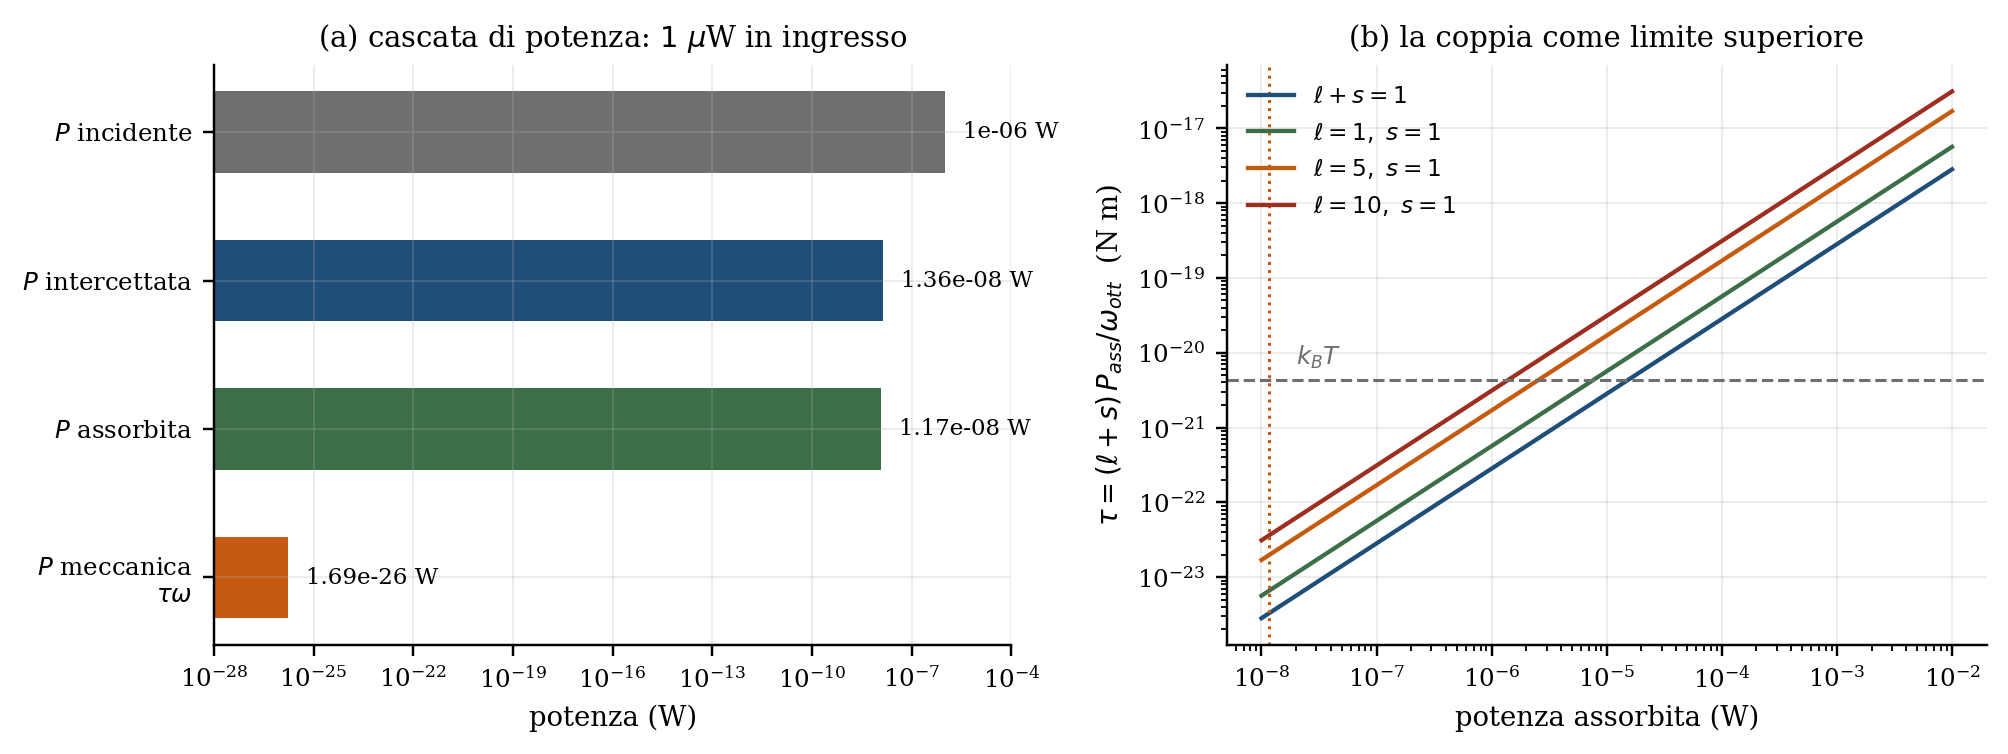
\includegraphics[width=\textwidth]{../figure/fig01_modello.png}
\caption{\textbf{(a)} The power cascade at \SI{1}{\micro W} input: $1.36$\,\%
intercepted, $86$\,\% of that absorbed, and the extracted mechanical power,
$1.7\times10^{-26}$\,W. \textbf{(b)} Torque \eqref{eq:modello} against absorbed power
for four values of $\ell+s$; the dashed line is $k_BT$.}
\label{fig:modello}
\end{figure}

\begin{table}[H]
\centering\small
\caption{Power budget at \SI{1}{\micro W} incident, $w_0=\SI{500}{nm}$.}
\label{tab:potenza}
\begin{tabular}{lrl}
\toprule
Quantity & Value & note \\
\midrule
$P_{\rm inc}$ & \SI{1}{\micro W} & reference power \\
$P_{\rm int}=I\sigma_{\rm pr}$ & \SI{13.56}{nW} & $1.356$\,\% of the beam \\
$P_{\rm abs}=I\sigma_{\rm abs}$ & \SI{11.70}{nW} & $86.3$\,\% of the intercepted \\
$P_{\rm sca}$ & \SI{1.85}{nW} & carried away without torque \\
$\tau=(\ell+s)P_{\rm abs}/\omega_{\rm ott}$ & $3.305\times10^{-24}$\,N\,m & V5: $2.610$ \\
$P_{\rm mech}=\tau\omega_{\rm ss}$ & $1.7\times10^{-26}$\,W & efficiency $1.4\times10^{-18}$ \\
\bottomrule
\end{tabular}
\end{table}

The last row is the harshest. The ratio of extracted mechanical power to absorbed
power is $1.4\times10^{-18}$: the device is not a machine converting light into
rotation, it is a resistor that heats. This depends neither on geometry nor on the
torque model, but on $\omega_{\rm ss}\ll\omega_{\rm ott}$: the photons are $10^{15}$
times ``faster'' than the rotor. An optical rotor can be an excellent torque sensor,
and it is: it cannot be an actuator.

%=====================================================================
\section{Optical audit}
\label{sec:ottica}
%=====================================================================

\subsection{The wire radius, and why it changes everything}

V5 declared a ``6.4 nm diameter'' for the orbit wires and then computed the size
parameter with $a=\SI{1.25}{nm}$. In the Rayleigh regime a cylinder's cross-section is
proportional to $a^2$, so the error was a factor 6.5 on the orbits, 36 on the rim ring
and 13 on the lenses. Redone with the scene radii --- 3.2, 7.5 and 4.5 nm --- the wire
contribution goes from 3\,\% to 34\,\% of the total cross-section, the mass from
$2.78$ to $8.21\times10^{-18}$\,kg and the moment of inertia from $3.1\times10^{-32}$
to $4.6\times10^{-31}$\,kg\,m$^2$. These are the differences between
Table~\ref{tab:confronto} and Table~\ref{tab:residui}. Nothing else in the optical
model changes: the form of the equations was not wrong, the geometry was.

\subsection{Models used and their status}

\begin{table}[H]
\centering\small
\caption{Status of the optical models. ``Exact'' means solution of Maxwell's equations
for that geometry; ``verified'' means checked against its own analytic limit.}
\label{tab:ottica}
\begin{tabular}{p{3.4cm}p{3.0cm}p{2.8cm}p{4.6cm}}
\toprule
Element & model & status & check \\
\midrule
Core \SI{40}{nm} & exact Mie & exact & $Q_{\rm ext}\ge Q_{\rm sca}$ over the whole range \\
Wires 6.4/15/9\,nm & cylindrical series $n\ge1$ & exact to $<1$\,\% & against Rayleigh: $0.3$\,\% at $x=0.038$ \\
Wire limit & cylindrical Rayleigh & analytic & used for $x<0.05$ \\
Oxide shell & quasi-static Maxwell-Garnett & approximate & limits $f\to0,1$ exact \\
$\varepsilon(a)$ & Drude with $\gamma=\gamma_b+Av_F/a$ & approximate & compared with bulk \\
Assembly & incoherent sum & \emph{assumption} & coherent bound $N^2\sigma_1$ declared \\
\bottomrule
\end{tabular}
\end{table}

The $n=0$ term of the Bohren-Huffman cylindrical formulae is unstable as $x\to0$: at
$x=0.015$ it yields $Q_{\rm ext}=0.138$ instead of $0.011$, an artefact of the
logarithmic divergence of $H_0$. The V6 series starts at $n=1$ and matches Rayleigh to
$0.3$\,\%. An implementer trusting the ``complete formula'' would have overestimated
the torque by a factor 13.

\subsection{Size dependence and oxidation}

The Drude correction $\gamma(a)=\gamma_{\rm bulk}+Av_F/a$ ($v_F=1.57\times10^6$\,m/s,
$\tau_{\rm bulk}=\SI{27}{fs}$) changes $Q_{\rm abs}$ by $1.4$\,\% at \SI{40}{nm}, by
$5$\,\% at \SI{10}{nm} and by $21$\,\% at \SI{2}{nm}: at \SI{532}{nm} copper is
dominated by interband transitions, not by the Drude term, and in the green it behaves
better than gold and silver.

A Cu$_2$O shell changes absorption monotonically: $+7.8$\,\% for \SI{0.7}{nm},
$+15.8$\,\% for \SI{1.4}{nm}, $+51$\,\% for \SI{5.4}{nm}, saturating beyond
\SI{8}{nm}. The effect goes in the ``more torque'' direction, but must be read with the
thermal balance: the same oxide raises emissivity and lowers the steady temperature.
In vacuum, oxidation is a thermal advantage before an optical one.

The dominant uncertainty is neither $\varepsilon(a)$ nor the oxide, but the dispersion
of the optical data: $\pm30$\,\% on $k$ shifts $\sigma_{\rm pr}$ by $-39/+44$\,\% and
$\sigma_{\rm abs}$ by $-47/+60$\,\%, while the same variation on $n$ gives
$-10/+6$\,\%. Anyone measuring this structure must first fix $k$.

\subsection{The assembly, and what is missing}

The frame cross-section is the incoherent sum of the cross-sections of the individual
elements: an assumption, valid if the distance between scatterers exceeds the lateral
coherence length of the beam and if near-field coupling is weak. At \SI{250}{nm}
spacing and $kD=3$ the assumption is reasonable but unproven; the rigorous upper bound
is $N^2\sigma_1$, a factor 4 above. A DDA/FDTD check of the whole frame remains open,
and it is the only point of V6 where an external calculation can change a number in
the text.

\begin{figure}[H]
\centering
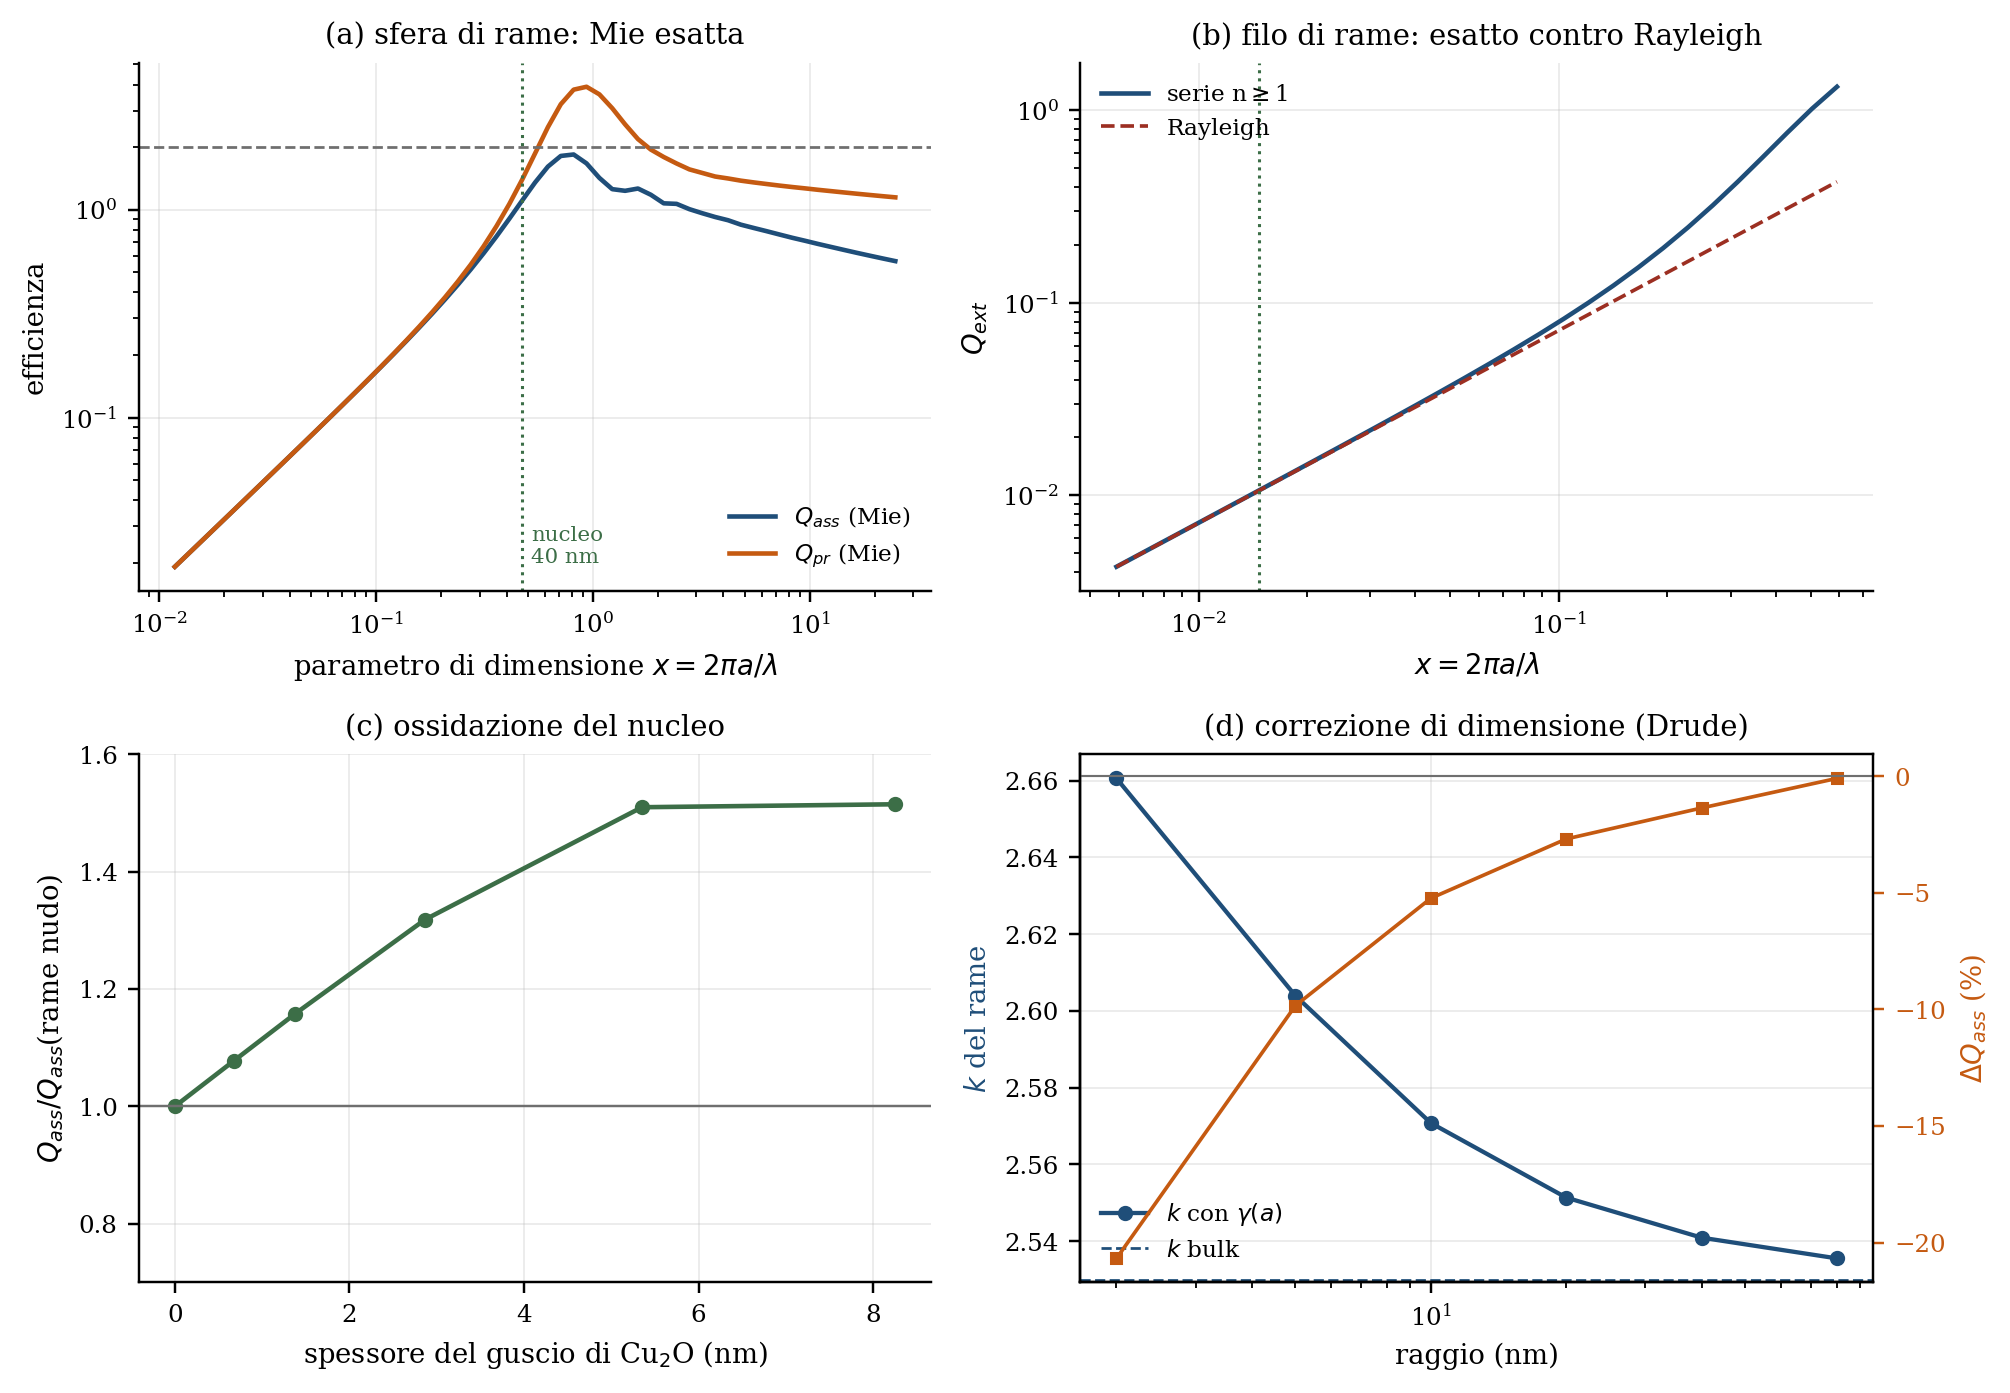
\includegraphics[width=\textwidth]{../figure/fig02_ottica.png}
\caption{\textbf{(a)} Mie efficiencies for a copper sphere: the \SI{40}{nm} core sits
at $x=0.47$, where $Q_{\rm pr}=1.40$ and $Q_{\rm abs}=1.11$. \textbf{(b)} The
cylindrical series against the Rayleigh limit: they coincide up to $x\approx0.05$; the
wires lie in the agreement region. \textbf{(c)} Effect of a Cu$_2$O shell.
\textbf{(d)} Drude correction: $k$ grows as the radius shrinks, but at \SI{40}{nm} the
effect on $Q_{\rm abs}$ is $1.4$\,\%.}
\label{fig:ottica}
\end{figure}

%=====================================================================
\section{Thermal balance}
\label{sec:termica}
%=====================================================================

The missing balance is one line, $P_{\rm abs}=P_{\rm diss}+P_{\rm out}$, and it closes
immediately: $P_{\rm diss}=\beta\omega_{\rm ss}^2=1.7\times10^{-26}$\,W, i.e.
$10^{-18}$ of the absorbed power. In steady state \emph{all} absorbed power leaves as
heat, and there are two paths: conduction into the medium and radiation.

In the fluid, with unit Nusselt number (at these scales $Ra\sim10^{-18}$):
\begin{equation}
\Delta T_{\rm fluid}=\frac{P_{\rm abs}}{4\pi\kappa_m r}=\SI{0.026}{K}
\quad\text{at \SI{1}{\micro W}.}
\end{equation}
Local boiling is reached at \SI{3.9}{mW}. In water the thermal problem does not exist.

In vacuum it dominates, and the delicate point is the area. The exposed metal surface
is $A=2\pi\sum a_iL_i+4\pi r_{\rm core}^2=2.69\times10^{-13}$\,m$^2$, six times less
than the spherical envelope $4\pi R_{\rm out}^2$ used in 6.0:
\begin{equation}
T=\left(T_0^4+\frac{P_{\rm abs}}{\epsilon\sigma_{\rm SB}A}\right)^{1/4}.
\end{equation}
At \SI{1}{\micro W} this gives \SI{2250}{K} with $\epsilon=0.03$ and \SI{1505}{K} with
$\epsilon=0.15$: in both cases the rotor has passed the melting point of copper
(\SI{1358}{K}). The incident power that leads to melting is
\SI{0.132}{\micro W} and \SI{0.662}{\micro W}; the adiabatic melting time is
\SI{0.28}{ms}, against a vacuum spin-up that requires \SI{24}{s}
(Table~\ref{tab:regimi}). This is the most robust result of the revision: in vacuum
the bottleneck is not torque, it is temperature, and geometry cannot negotiate it.

On emissivity it is worth being explicit, because 6.0 used $\epsilon=0.6$. The
emissivity of a subwavelength object depends on volumetric absorption at
\SI{10}{\micro m}, not on the bulk optical constant of a thin oxide: a \SI{1.4}{nm}
Cu$_2$O shell does not bring the object to $\epsilon=0.6$. V6 uses the interval
$0.03$--$0.15$ and shows that even the upper end does not save the rotor.

\begin{table}[H]
\centering\small
\caption{Thermal balance of the reference configuration. The last column is the
adiabatic time to reach $T_m$.}
\label{tab:termica}
\begin{tabular}{rrrrrr}
\toprule
$P_{\rm inc}$ & $P_{\rm abs}$ & $\Delta T$ water & $T$ vacuum ($\epsilon=0.03$) & $T$ vacuum ($\epsilon=0.15$) & $t_{\rm ad}$ \\
\midrule
\SI{1}{\micro W} & \SI{11.7}{nW} & \SI{0.026}{K} & \SI{2250}{K} & \SI{1505}{K} & \SI{0.28}{ms} \\
\SI{100}{\micro W} & \SI{1.17}{\micro W} & \SI{2.6}{K} & \SI{7113}{K} & \SI{4757}{K} & \SI{2.8}{\micro s} \\
\SI{10}{mW} & \SI{117}{\micro W} & \SI{258}{K} & \SI{22495}{K} & \SI{15043}{K} & \SI{28}{ns} \\
\bottomrule
\end{tabular}
\end{table}

Two operational consequences. First: in vacuum emissivity is a first-order design
variable, more than geometry. Second: pulsed operation, which V5 treated as a dynamical
regime, is the only way to work in vacuum at high power; the duty cycle is
$P_{\rm fus}/P_{\rm abs}$ at peak power.

\begin{figure}[H]
\centering
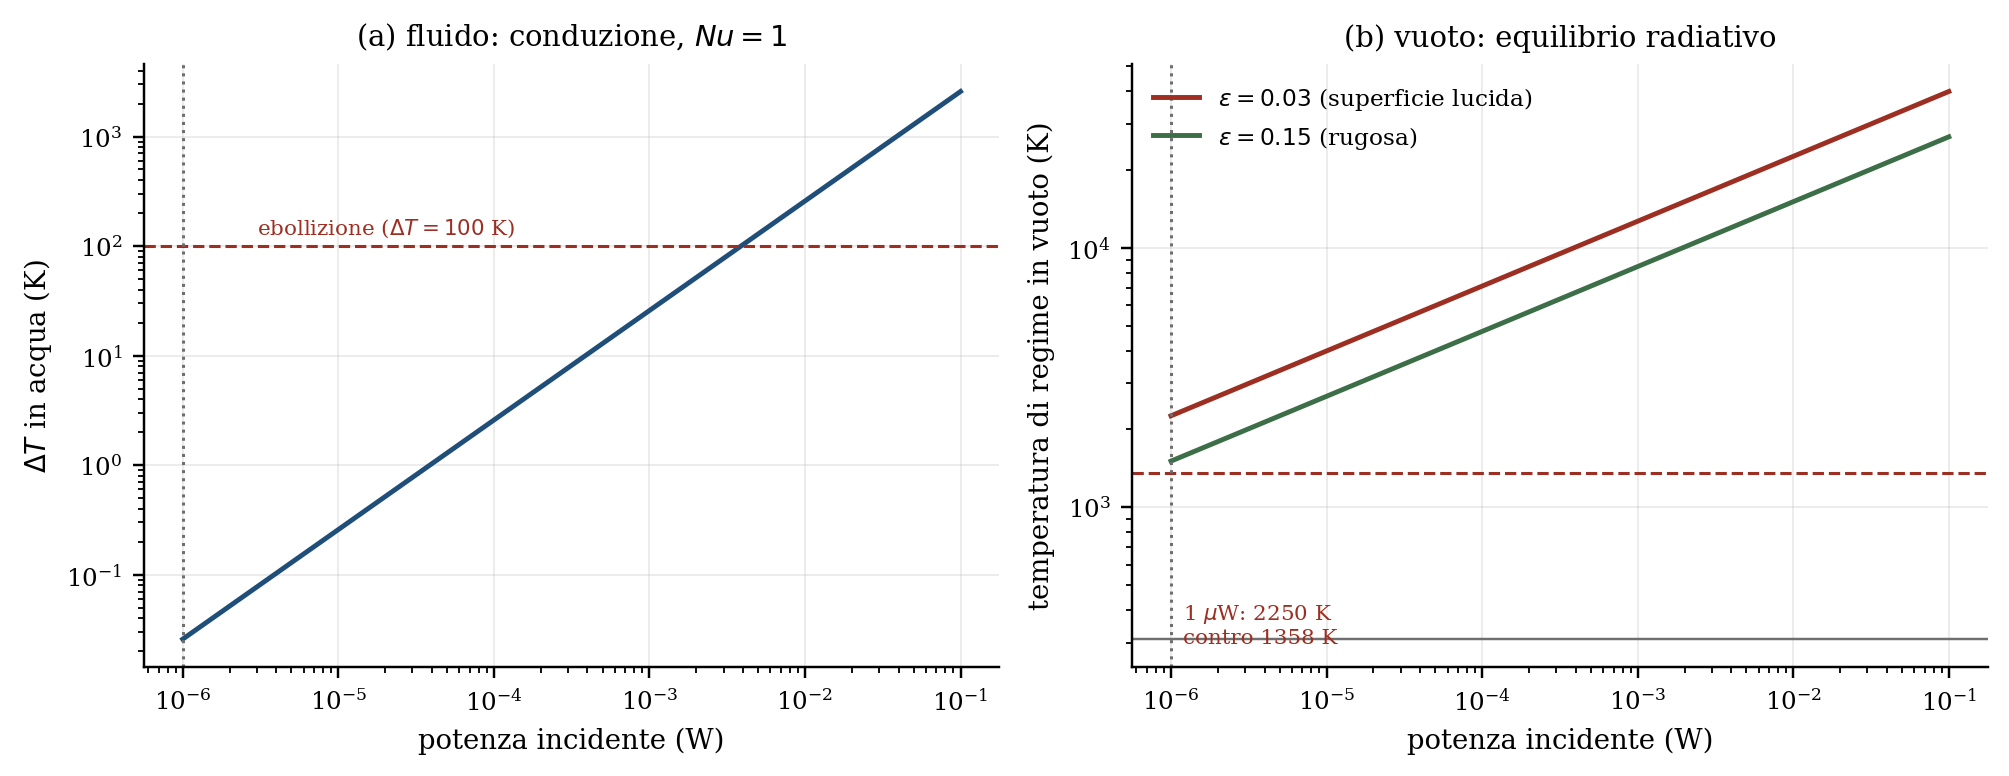
\includegraphics[width=\textwidth]{../figure/fig03_termica.png}
\caption{\textbf{(a)} Heating in water: \SI{0.026}{K} at \SI{1}{\micro W}, boiling at
\SI{3.9}{mW}. \textbf{(b)} Radiative equilibrium with the real metal surface: at
\SI{1}{\micro W} both emissivities exceed melting.}
\label{fig:termica}
\end{figure}

%=====================================================================
\section{Equal-mass baseline}
\label{sec:baseline}
%=====================================================================

This section answers the question ``what do the lenses and the Counter-spin add''. The
comparison is at constant mass ($8.211\times10^{-18}$\,kg), constant power
(\SI{1}{\micro W}), constant wavelength and medium.

\begin{table}[H]
\centering\footnotesize
\setlength{\tabcolsep}{3.5pt}
\caption{Six geometries at equal mass, $P=\SI{1}{\micro W}$, $w_0=\SI{500}{nm}$.
$\sigma_{abs}$ is the cross-section used: for the lattice the element-by-element
calculation, for the others the equal-volume sphere; $Pe_r$ and $\omega_{ss}$ report
the optical interval declared in the text. $t_r$ is the vacuum breaking time.}
\label{tab:baseline}
\begin{tabular}{lrrrrrrr}
\hline
Geometry & $R$ (nm) & $\beta$ (N\,m\,s) & $\sigma_{abs}$ (m$^2$) & $\tau$ (N\,m) & $Pe_r$ & $\omega_{ss}$ (rad/s) & $t_{r}$ (s) \\
\hline
Lattice (V5) & 370 & $4.04$--$6.48\times10^{-22}$ & $9.19\times10^{-15}$ & $3.31\times10^{-24}$ & $7.72\times10^{-4}$ & $5.10$--$8.19\times10^{-3}$ & $56.4$ \\
Solid disc & 143 & $3.73\times10^{-23}$ & $2.07\times10^{-14}$ & $7.44\times10^{-24}$ & $1.74$--$5.22\times10^{-3}$ & $0.199$--$0.598$ & $11.8$ \\
Ring & 420 & $7.21$--$9.51\times10^{-22}$ & $2.07\times10^{-14}$ & $7.44\times10^{-24}$ & $1.74$--$5.22\times10^{-3}$ & $7.83\times10^{-3}$--$0.031$ & $69.3$ \\
Sphere & 60 & $6.60\times10^{-24}$ & $2.07\times10^{-14}$ & $7.44\times10^{-24}$ & $1.74\times10^{-3}$ & $1.13$ & $3.97$ \\
Nanodumbbell & 143 & $2.64$--$3.30\times10^{-23}$ & $2.07\times10^{-14}$ & $7.44\times10^{-24}$ & $1.74$--$5.22\times10^{-3}$ & $0.226$--$0.846$ & $11.6$ \\
Anisotropic silica & 96 & $2.69\times10^{-23}$ & $1.01\times10^{-20}$ & $6.68\times10^{-27}$ & $1.56$--$4.68\times10^{-6}$ & $2.49$--$7.46\times10^{-4}$ & $7.1\times10^{3}$ \\
\hline
\end{tabular}

\end{table}

\begin{figure}[H]
\centering
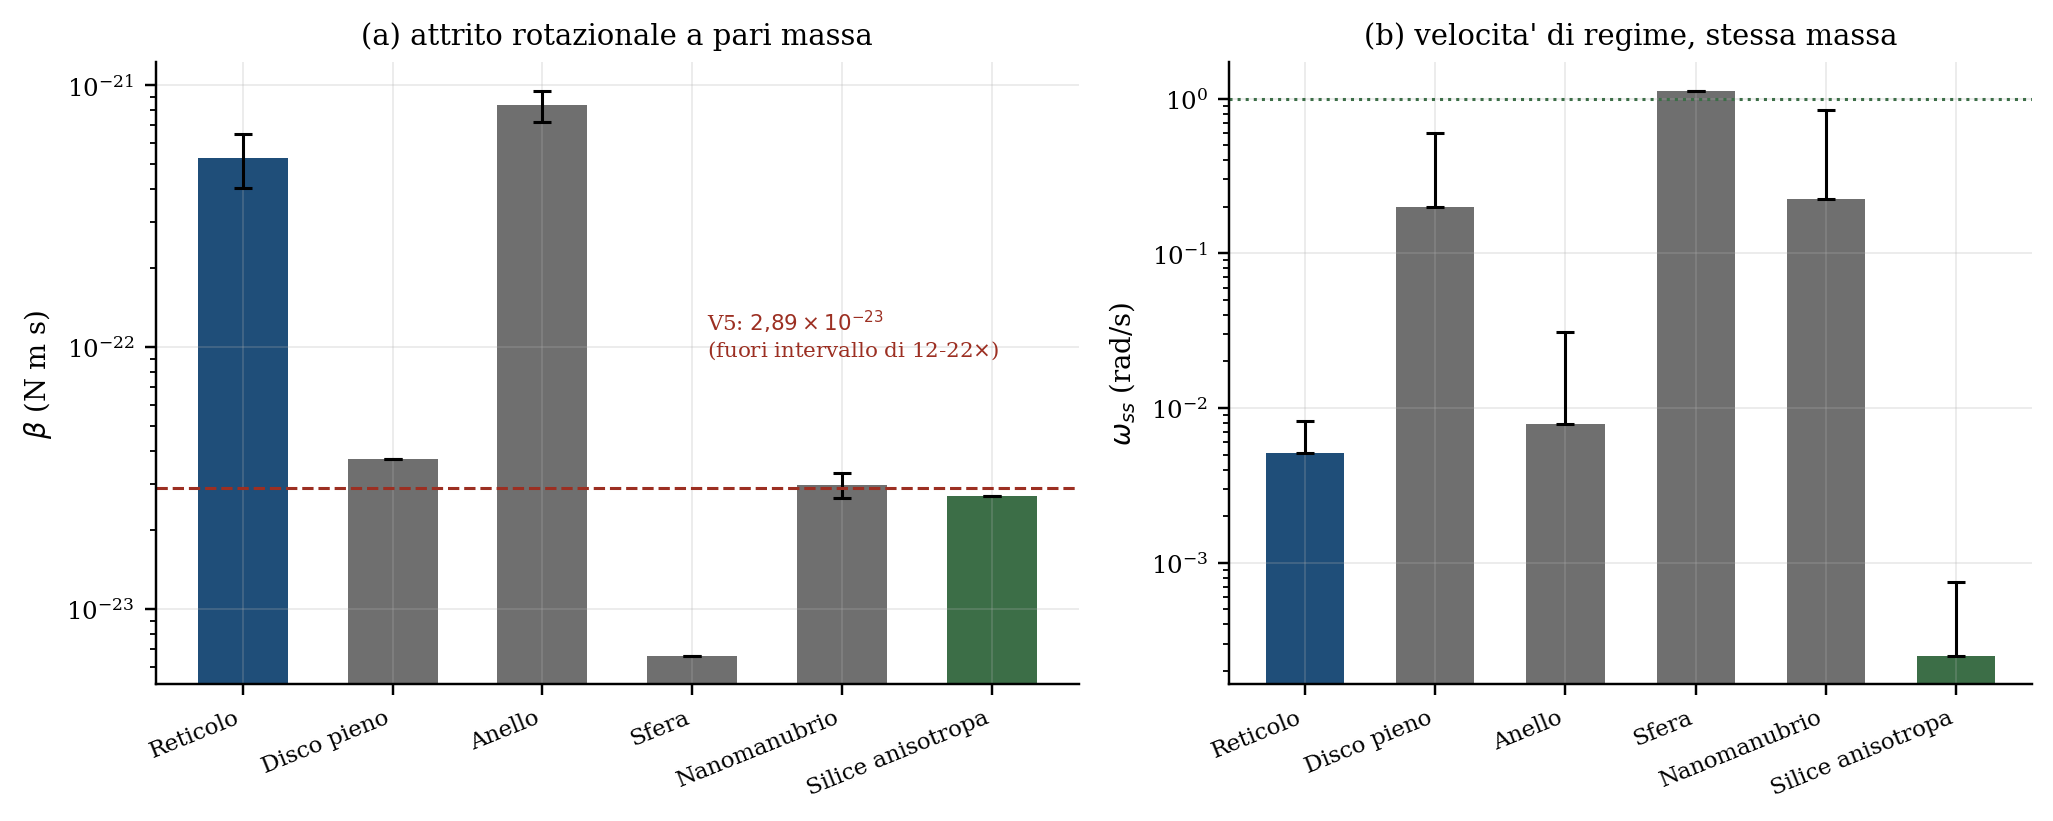
\includegraphics[width=\textwidth]{../figure/fig04_baseline.png}
\caption{\textbf{(a)} Rotational drag of the six geometries, with the physical interval
for slender bodies; the red line is the V5 estimate. \textbf{(b)} Steady rotation rate
with the optical band declared in the text.}
\label{fig:baseline}
\end{figure}

\subsection{Torque is not a result: it is a declared assumption}

In 6.0 every geometry received the equal-volume sphere cross-section, and $Pe_r$ came
out identical by construction. That was an assumption dressed as a result, and 6.1
corrects it in two ways.

First, the lattice uses \emph{its own} cross-section, computed element by element:
$\sigma_{\rm abs}=9.19\times10^{-15}$\,m$^2$, corresponding to
$Pe_r=7.72\times10^{-4}$. The compact sphere of equal mass ($r=\SI{60}{nm}$) absorbs
$2.07\times10^{-14}$, 125\,\% more, giving $Pe_r=1.74\times10^{-3}$. The difference is
physical and is explained in one line: in the Rayleigh limit absorption is proportional
to volume, but the core sits at $x=0.47$ and the equivalent sphere at $x=0.71$, a
region where $Q_{\rm abs}$ grows with size. By spreading the same material into thin
wires, the lattice loses the resonance gain.

Second, for disc, ring and dumbbell the cross-section is given as a \emph{band}: one to
three times the equal-volume value, because shape resonances at fixed volume shift
$Q_{\rm abs}$ by a factor 2--3 and a real estimate requires a DDA calculation per
shape. Table~\ref{tab:baseline} reports the interval, and the optical conclusion must
be read as conditional: \emph{if} the cross-section stays within three times the
volume value, then at equal mass none of these geometries gains more than a factor 3
in $Pe_r$.

For drag, on the other hand, the result is not conditional: $\beta$ ranges from
$6.6\times10^{-24}$ (sphere) to $8.4\times10^{-22}$ (ring), two decades, and is
computed per shape. This is the part that holds.

\subsection{What the wires, the lenses and the Counter-spin actually do}

The decomposition of the lattice, with the corrected wire radii:
\begin{center}\small
\begin{tabular}{lrrr}
\toprule
component & mass share & share of $\sigma_{\rm abs}$ & share of $\beta$ \\
\midrule
spherical core \SI{40}{nm} & 29.3\,\% & 60.6\,\% & 0.5\,\% \\
frame (orbits, rim, lenses) & 70.7\,\% & 39.4\,\% & 99.5\,\% \\
\bottomrule
\end{tabular}
\end{center}
With the scene wire radii the frame is no longer optically marginal: it carries 39\,\%
of the torque. It remains, however, a drag multiplier of 209 with respect to the bare
core. If its role were optical it would be a trade-off; if the role is mechanical ---
holding the core on axis, distributing mass, setting the moment of inertia --- it must
be judged on that, and V6 finds no measurement that justifies it at this scale.

The Counter-spin belongs in the appendix with 45/376. Here the quantitative consequence
suffices: it adds moment of inertia and drag without adding torque. Maintaining the
ratio requires a mechanical constraint, and a mechanical constraint between two rotors
makes them a single rigid body.

\subsection{The alternative structure}

Two variants emerge. The \emph{solid disc} at equal mass ($R=\SI{143}{nm}$,
$t=\SI{14}{nm}$) has $\omega_{\rm ss}$ 39 times larger than the lattice and no
optically useless element. \emph{Anisotropic silica} is the only geometry that changes
the physical channel: it does not absorb ($\sigma_{\rm abs}=1.0\times10^{-20}$\,m$^2$)
and works by phase retardation, $\tau=(P_{\rm int}/\omega_{\rm ott})\sin^2(\delta/2)$;
at \SI{1}{\micro W} in water it gives $6.7\times10^{-27}$\,N\,m, four hundred times
less than copper; in vacuum at high power it is the only one that does not melt. The
conclusion is not that copper is better: it is that \emph{the torque channel must be
chosen together with the medium}, and V6 shows this instead of assuming it.

\begin{figure}[H]
\centering
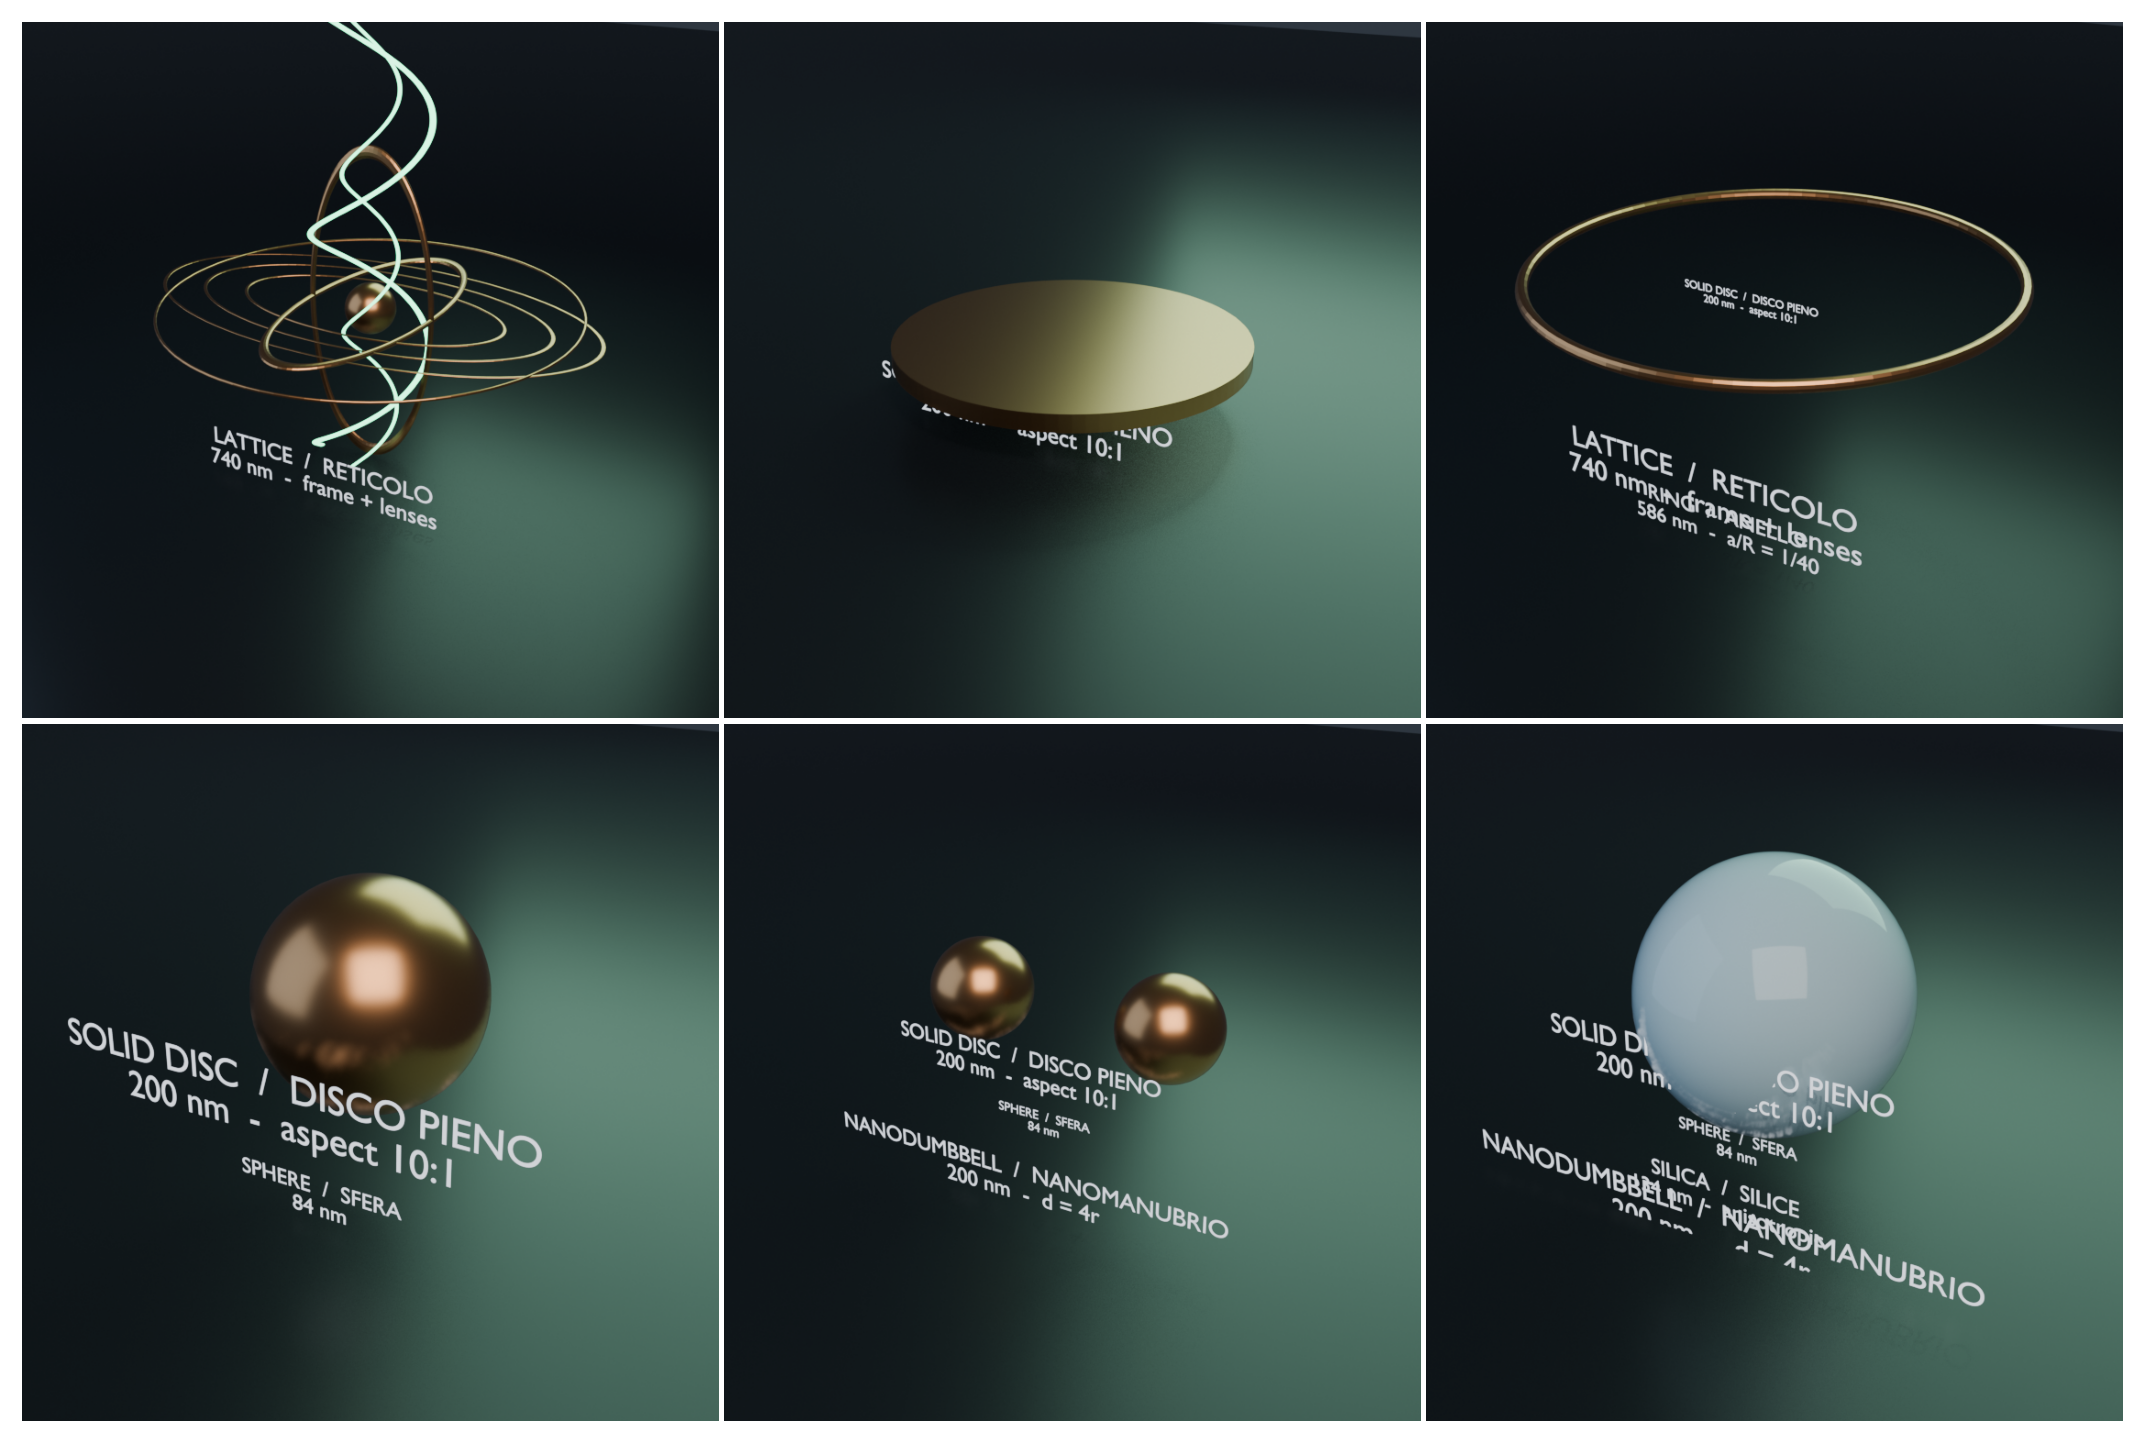
\includegraphics[width=\textwidth]{../figure/fig11_baseline_render.png}
\caption{The six geometries at equal mass, rendered at the same apparent size (the real
size is in each panel caption). The scale difference is the point: the same mass,
spread over a \SI{740}{nm} frame or packed into an \SI{84}{nm} sphere, changes $\beta$
by two decades and $Pe_r$ by a factor 2.}
\label{fig:render_baseline}
\end{figure}

%=====================================================================
\section{Regime matrix}
\label{sec:regimi}
%=====================================================================

The matrix crosses four external sizes with two media. The scale factor is
$s=L/2R_{\rm out}$, so the ``240 nm'' column describes a reduced frame, not the
reference configuration.

\begin{table}[H]
\centering\footnotesize
\setlength{\tabcolsep}{3.5pt}
\caption{Regime matrix: four sizes $L$ and two media, $P=\SI{1}{\micro W}$. In vacuum
$\omega_{ss}$ does not exist (``--'') and the breaking time takes its place. $T$ is the
steady temperature with $\epsilon=0.15$; at \SI{1}{\micro W} it already exceeds the
melting point of copper.}
\label{tab:regimi}
\begin{tabular}{llrrrrrrl}
\hline
$L$ & medium & $\eta_{int}$ & $\tau$ (N\,m) & $\omega$ (rad/s) & $Pe_r$ & $t_{rupt}$ (s) & $T$ (K) & validity \\
\hline
1 nm & fluid & $9.90\times10^{-8}$ & $2.41\times10^{-29}$ & $1.89$--$3.03$ & $5.64\times10^{-9}$ & -- & 310 & out of domain \\
1 nm & vacuum & $9.90\times10^{-8}$ & $2.41\times10^{-29}$ & -- & $5.64\times10^{-9}$ & $4.1\times10^{-4}$ & 1505 & out of domain \\
240 nm & fluid & $5.70\times10^{-3}$ & $1.39\times10^{-24}$ & $7.86\times10^{-3}$--$0.0126$ & $3.25\times10^{-4}$ & -- & 310 & valid \\
240 nm & vacuum & $5.70\times10^{-3}$ & $1.39\times10^{-24}$ & -- & $3.25\times10^{-4}$ & $23.7$ & 1505 & valid \\
1 $\mu$m & fluid & $0.099$ & $2.41\times10^{-23}$ & $1.89$--$3.03\times10^{-3}$ & $5.64\times10^{-3}$ & -- & 310 & valid \\
1 $\mu$m & vacuum & $0.099$ & $2.41\times10^{-23}$ & -- & $5.64\times10^{-3}$ & $412$ & 1505 & valid \\
1 m & fluid & $1$ & $2.82\times10^{-22}$ & $2.21\times10^{-20}$ & $0.066$ & -- & 310 & valid \\
1 m & vacuum & $1$ & $2.82\times10^{-22}$ & -- & $0.066$ & $3.5\times10^{25}$ & 310 & extrapolation \\
\hline
\end{tabular}

\end{table}

\begin{figure}[H]
\centering
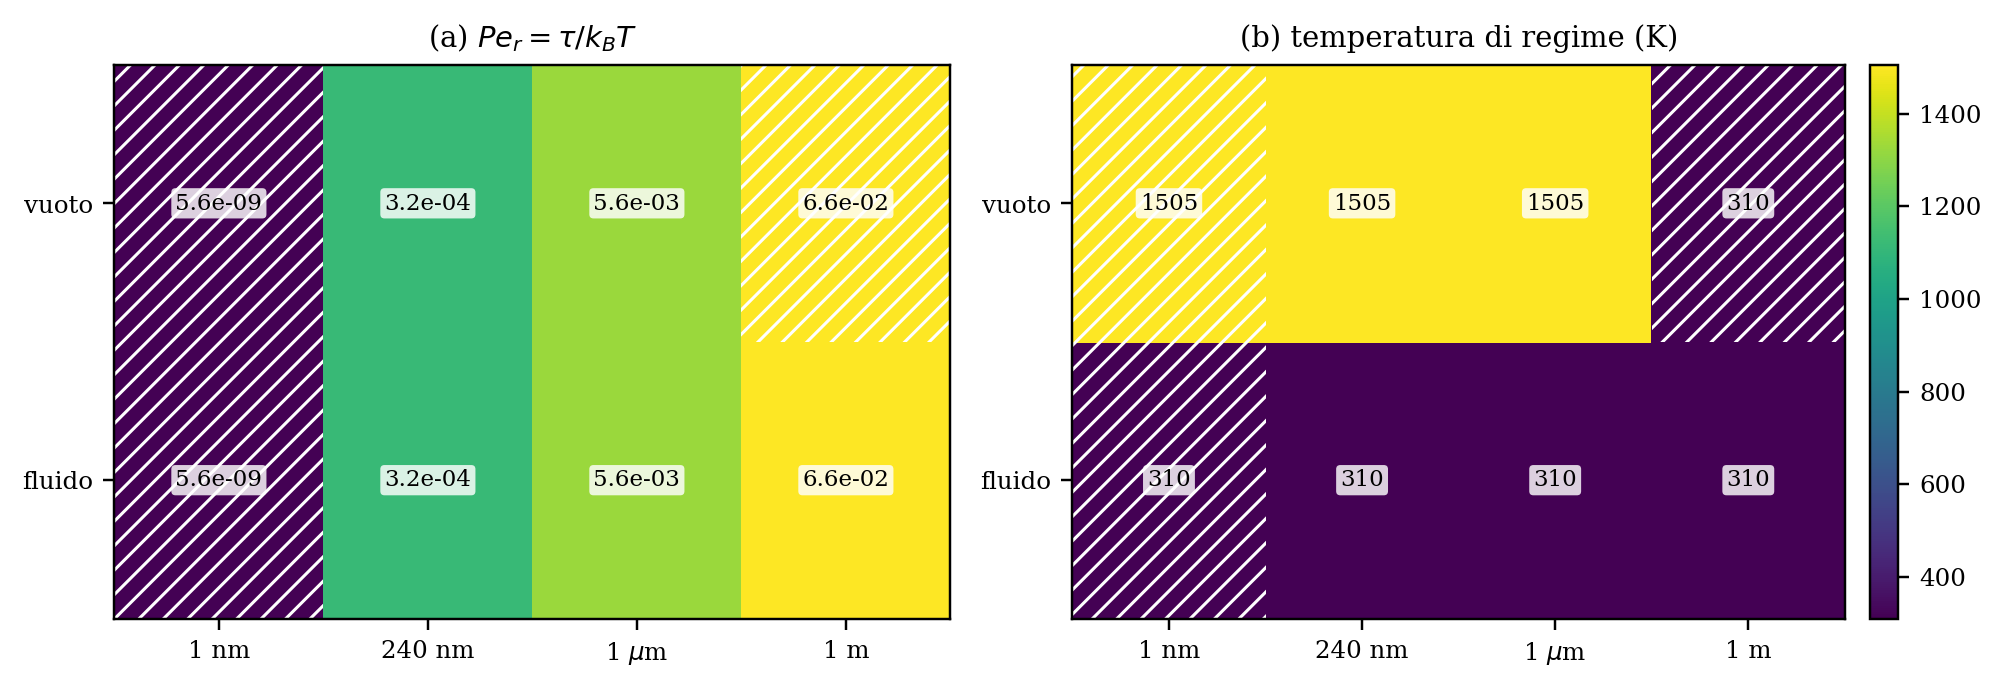
\includegraphics[width=\textwidth]{../figure/fig05_regimi.png}
\caption{Regime matrix: $Pe_r$ and steady temperature. Hatched cells lie outside the
domain of validity (sub-atomic wire at \SI{1}{nm}, extrapolation at \SI{1}{m}).}
\label{fig:regimi}
\end{figure}

Three readings.

\textbf{Scale.} $Pe_r\propto\sigma_{\rm abs}\propto L^2$ as long as the structure is
smaller than the beam, then saturates at $P/(\omega_{\rm ott}k_BT)=0.066$. There is no
privileged scale for torque: a large geometry does not gain in $Pe_r$, it loses in
$\beta$.

\textbf{Medium.} In a fluid a steady state exists; in vacuum it does not. In vacuum the
relevant quantity is the breaking time, $t_r=I\omega_{\rm lim}/\tau$: \SI{24}{s} at
\SI{240}{nm}, \SI{410}{s} at \SI{1}{\micro m}. Temperature, by contrast, does not depend
on scale in the Rayleigh regime ($P_{\rm abs}\propto R^2$ and $A\propto R^2$): it stays
at \SI{1505}{K} at every size until interception saturates. Shrinking the rotor does
not cool it.

\textbf{Validity.} The two extreme columns are not physics. At \SI{1}{nm} the wire would
have a radius of \SI{8.6}{pm}, less than a copper atom (\SI{0.13}{nm}), and the
continuum does not apply; at \SI{1}{m} Reynolds number and gravity change the problem.
V6 flags them instead of presenting them as ``invariance over nine orders of
magnitude'': the geometric invariance of the 45/376 ratio is real, that of the physical
behaviour is not.

%=====================================================================
\section{Materials}
\label{sec:materiali}
%=====================================================================

\begin{table}[H]
\centering\scriptsize
\setlength{\tabcolsep}{3pt}
\caption{Same geometry, three materials. $T$ is the steady temperature in vacuum at
\SI{1}{\micro W} with $\epsilon=0.15$; the margin is $T_m/T$.}
\label{tab:materiali}
\begin{tabular}{lrrrrrrrrr}
\hline
Material & $\rho$ & $\sigma_y$ (MPa) & $\sigma_y/\rho$ (m$^2$/s$^2$) & $v_{lim}$ (m/s) & $Q_{abs}$ & $\sigma_{abs}$ (m$^2$) & $Pe_r$ & $T$ vacuum (K) & margin \\
\hline
Copper & 8960 & 200 & $2.2\times10^{4}$ & 149 & 1.11 & $9.19\times10^{-15}$ & $7.72\times10^{-4}$ & 1505 & 0.90 \\
Fused silica & 2200 & 1000 & $4.5\times10^{5}$ & 674 & 0.00 & $1.46\times10^{-21}$ & $1.23\times10^{-10}$ & 310 & 6.40 \\
Graphene / CNT & 1300 & 20000 & $1.5\times10^{7}$ & 3922 & 0.77 & $7.52\times10^{-15}$ & $6.32\times10^{-4}$ & 944 & 4.13 \\
\hline
\end{tabular}

\end{table}

\begin{figure}[H]
\centering
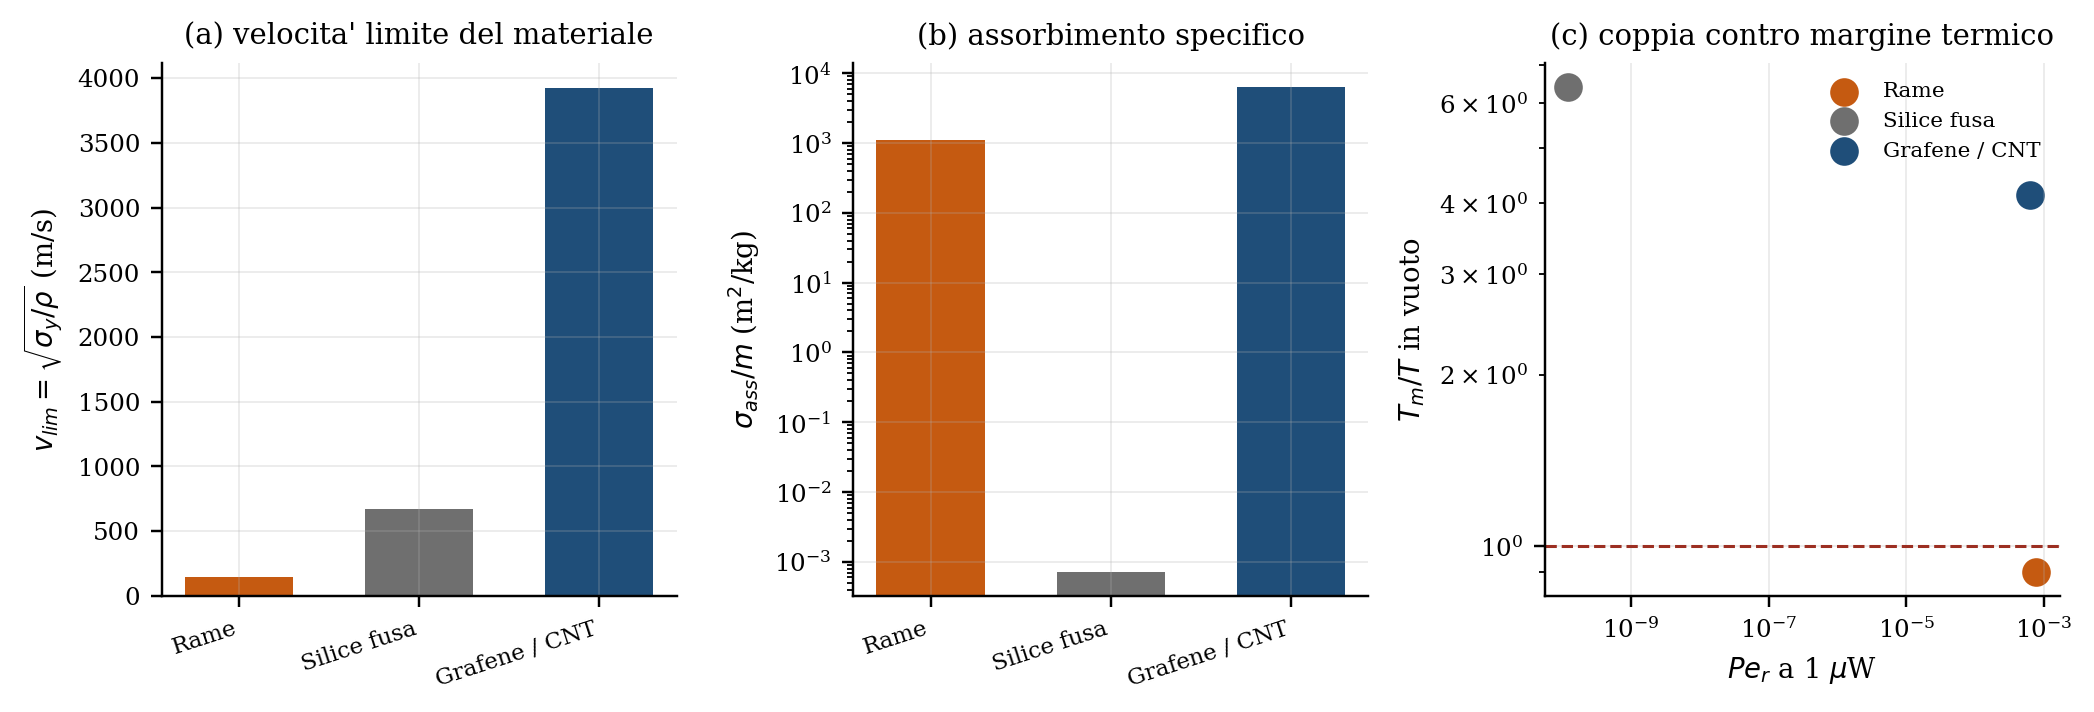
\includegraphics[width=\textwidth]{../figure/fig06_materiali.png}
\caption{\textbf{(a)} Limiting speed $\sqrt{\sigma_y/\rho}$, the only quantity that sets
the rotation ceiling in vacuum. \textbf{(b)} Specific absorption: copper wins.
\textbf{(c)} The real trade-off: more torque means less thermal margin.}
\label{fig:materiali}
\end{figure}

Copper wins on specific absorption by a factor 1.2 over graphene and $10^{10}$ over
silica; graphene wins on limiting speed by a factor 26 over copper; silica wins on
thermal margin and loses on everything else. There is no best material: there is the
right material for the chosen channel.

For graphene the ``absorption'' entry needs care. A single sheet absorbs $2.3$\,\% per
pass ($\pi\alpha$), and a few-layer structure reaches an absorption comparable to
copper; but in-plane thermal conductivity is \SI{3000}{W/m/K} against
\SI{401}{W/m/K}, and the internal gradient, negligible for copper, must be computed
here. V6 uses an effective density of 1300\,kg/m\textsuperscript{3} and an effective
strength of \SI{20}{GPa}: working values, not measurements, to be replaced with data
from the individual sample.

%=====================================================================
\section{Design levers}
\label{sec:leve}
%=====================================================================

\begin{table}[H]
\centering\small
\caption{Effect of each lever on the two figures of merit.}
\label{tab:leve}
\begin{tabular}{p{6.2cm}rrp{5.2cm}}
\hline
Lever & on $Pe_r$ & on $\omega_{ss}$ & note \\
\hline
Power $\times10$ (1 $\to$ 10\,$\mu$W) & $10$ $\times$ & $10$ $\times$ &  \\
Focusing NA 0.9 ($w_0$ 500 $\to$ 361 nm) & $1.92$ $\times$ & $1.92$ $\times$ &  \\
Linear polarization ($s=0$) & $0$ $\times$ & $0$ $\times$ &  \\
OAM $\ell=5$ with $s=1$ (mode overlap included) & $1.05$ $\times$ & $1.05$ $\times$ &  \\
Compaction at equal mass ($R/10$) & $1$ $\times$ & $290$ $\times$ & torque unchanged; $\omega$ follows the drag ratio ($10^2$--$10^3$) \\
High vacuum ($p=10^{-6}$ mbar) & $1$ $\times$ & $1.33\times10^{10}$ $\times$ & no true steady state: fracture becomes the limit \\
Material: graphene instead of copper & $0.818$ $\times$ & $0.818$ $\times$ & specific absorption changes; effect on $Pe_r$ = 0.82 \\
\hline
\end{tabular}

\end{table}

\begin{figure}[H]
\centering
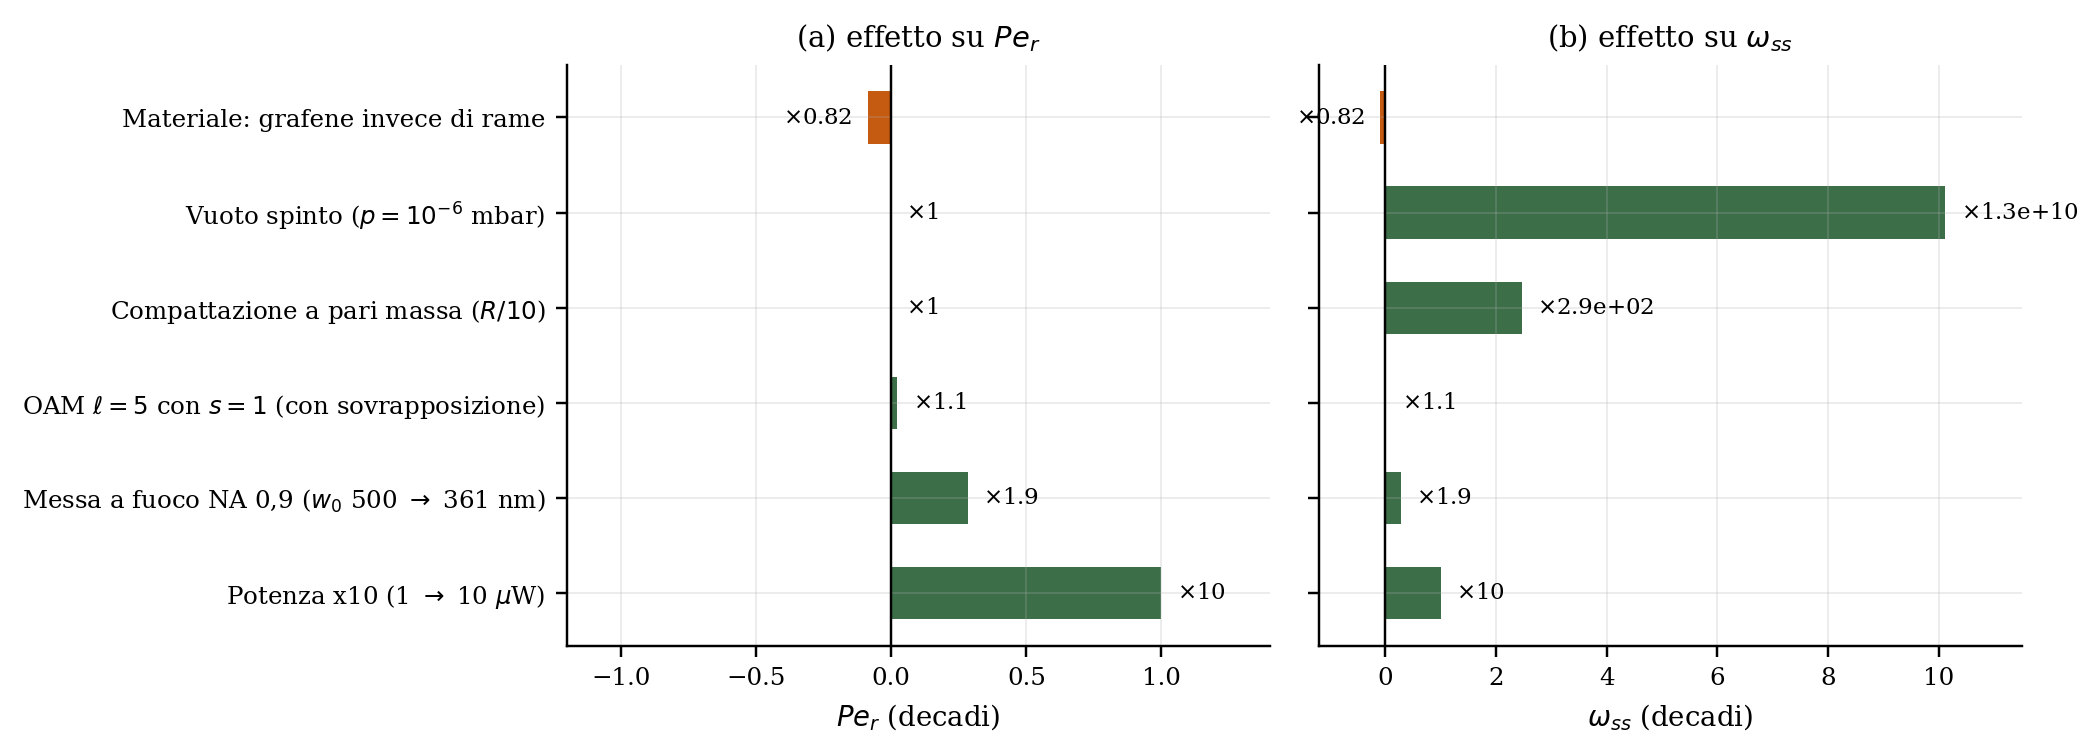
\includegraphics[width=\textwidth]{../figure/fig07_leve.png}
\caption{Effect of each lever on $Pe_r$ (a) and $\omega_{ss}$ (b). The two columns do
not coincide, and the difference is the message: compaction and vacuum change $\omega$
by ten decades and $Pe_r$ by zero.}
\label{fig:leve}
\end{figure}

The most effective lever is power, and that is no surprise: $Pe_r\propto P$. The second
is focusing, \SI{1.92}{}; the third is material, which however works against us
(graphene absorbs $0.82$ of copper at the same geometry). OAM, as \S\ref{sec:oam}
shows, is worth $1.05$ and not $6$: the table already includes the mode overlap, and
this is the most important correction with respect to 6.0.

The two ``free'' levers do not exist. Polarization is necessary, not multiplicative:
with $s=0$ and $\ell=0$ the torque is zero. Compaction is worth a factor 290 on
$\omega_{\rm ss}$ and zero on $Pe_r$: it improves the response without improving the
drive, which is exactly what a sensor needs.

%=====================================================================
\section{External check: silica at 1--6\,GHz}
\label{sec:ghz}
%=====================================================================

This section does not claim a validation. It separates two statements that 6.0 kept
together: order-of-magnitude compatibility on the \emph{mechanical scale}, and
validation of the \emph{optical model}. The first is verified, the second is not, and
no available datum supports it.

\begin{table}[H]
\centering\small
\caption{Mechanical ceiling $f_{\rm lim}=(2\pi r)^{-1}\sqrt{\sigma_y/\rho}$ in GHz, for
four radii and five values of the silica fracture strength.}
\label{tab:ghz}
\begin{tabular}{rrrrr}
\hline
$\sigma_y$ (GPa) & $r=25$ nm & $r=50$ nm & $r=75$ nm & $r=100$ nm \\
\hline
0.5 & $3.03$ & $1.52$ & $1.01$ & $0.759$ \\
1 & $4.29$ & $2.15$ & $1.43$ & $1.07$ \\
3 & $7.43$ & $3.72$ & $2.48$ & $1.86$ \\
5 & $9.6$ & $4.8$ & $3.2$ & $2.4$ \\
8 & $12.1$ & $6.07$ & $4.05$ & $3.03$ \\
\hline
\end{tabular}

\end{table}

\begin{table}[H]
\centering\small
\caption{The experimental records and the effective strength they imply,
$\sigma_y=\rho(2\pi rf)^2$ with $\rho=2200$\,kg/m$^3$.}
\label{tab:ghz_reg}
\begin{tabular}{rrrr}
\hline
$f$ (GHz) & $r$ (nm) & $v=2\pi r f$ (m/s) & $\rho v^2$ (GPa) \\
\hline
1 & 50 & 314 & 0.22 \\
1 & 75 & 471 & 0.49 \\
5 & 50 & 1571 & 5.43 \\
6 & 50 & 1885 & 7.82 \\
\hline
\end{tabular}

\end{table}

\begin{figure}[H]
\centering
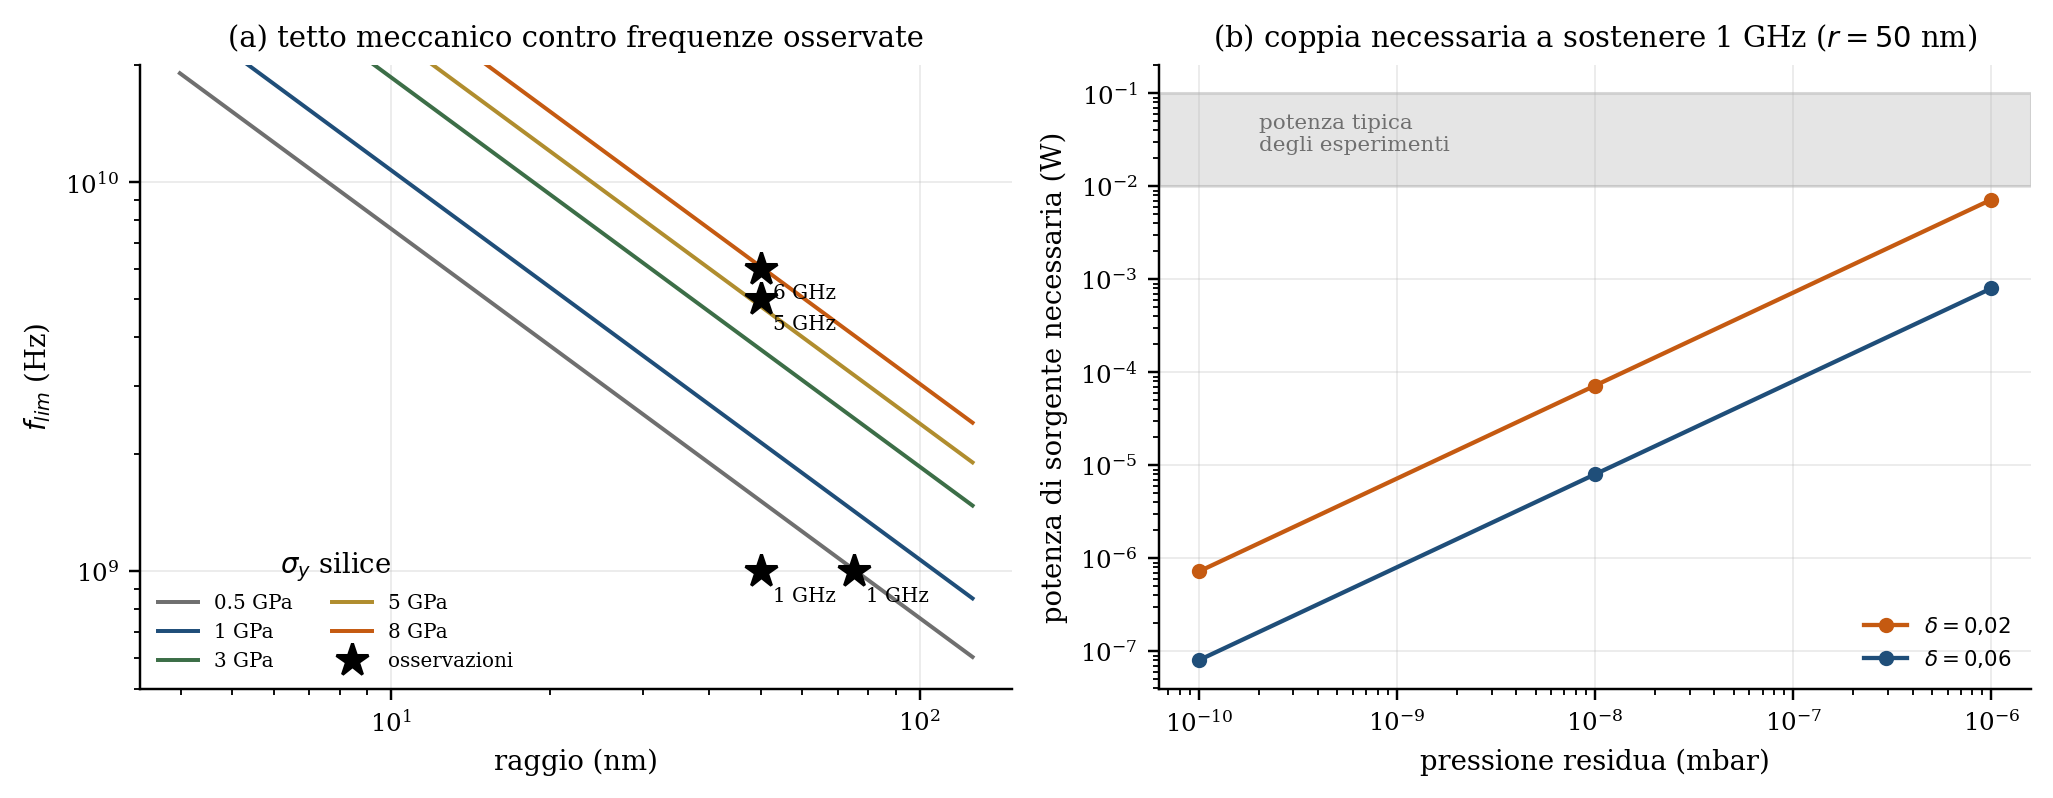
\includegraphics[width=\textwidth]{../figure/fig08_ghz.png}
\caption{\textbf{(a)} Mechanical ceiling for five values of $\sigma_y$; the stars are
the observed frequencies. Observations fall between 0.2 and 8\,GPa, i.e. in the range
of nanoscale silica. \textbf{(b)} Source power needed to sustain \SI{1}{GHz} against
molecular drag: far below the power used in the experiments, which serves the trap, not
the torque.}
\label{fig:ghz}
\end{figure}

\textbf{(1) Mechanical compatibility.} The reported $(f,r)$ pairs imply $\sigma_y$
between $0.22$\,GPa (\SI{1}{GHz} at \SI{50}{nm}) and $7.8$\,GPa (\SI{6}{GHz} at
\SI{50}{nm}). The formula reproduces the observed frequencies for values of $\sigma_y$
that are those expected for nanoscale silica, and this is a consistency check, not a
prediction: $\sigma_y$ was inferred from the observations, not measured independently.
A single point with a chosen $\sigma_y$ is not a validation; four points with $\sigma_y$
free are a constraint.

\textbf{(2) Torque is in surplus.} At \SI{1}{GHz} in vacuum at \SI{1e-6}{mbar} the
molecular drag on a \SI{50}{nm} sphere is $1.0\times10^{-27}$\,N\,m; \SI{0.8}{mW} of
source power suffice with $\delta=0.06$, and \SI{8}{\micro W} at \SI{1e-8}{mbar},
against the typical \SI{10}{}--\SI{100}{mW}. The difference is the optical trap. The
model predicts surplus torque, which is consistent with the experiment, but does not
prove it.

\textbf{(3) What is missing for validation.} One would need measured $\tau$ against
$P_{\rm abs}$ at known geometry, and the dependence of $\omega_{\rm ss}$ on $\beta$ at
variable medium. Neither is available for this device. The correct statement is
therefore: the comparison offers a preliminary external check on the mechanical scale,
not an experimental validation of the Photonic Engine.

%=====================================================================
\section{OAM as a sensitivity analysis}
\label{sec:oam}
%=====================================================================

6.0 treated $\ell$ as a multiplier: $\tau=(\ell+s)P_{\rm abs}/\omega_{\rm ott}$, so
$\ell=5$ is worth six times. That is wrong at fixed \emph{incident} power, because
$\eta_{\rm int}$ does not stay constant.

For an $LG_{0\ell}$ beam of power $P$ and waist $w_0$, the peak intensity, normalized
to the Gaussian, is
\begin{equation}
g(\ell)=\frac{\ell^{\ell}e^{-\ell}}{\ell!},
\qquad g(1)=0.368,\; g(5)=0.176,\; g(10)=0.125,
\end{equation}
and on axis it vanishes for $\ell\ge1$. A particle placed at the maximum intercepts
$\sigma I_{\rm peak}$, so the net torque scales as $(\ell+s)\,g(\ell)$:
\begin{center}\small
\begin{tabular}{lrrrrr}
\toprule
$\ell$ & 0 & 1 & 5 & 10 & 20 \\
\midrule
$g(\ell)$ & 1 & 0.368 & 0.176 & 0.125 & 0.089 \\
$\tau(\ell)/\tau(0)$ & 1 & 0.74 & 1.05 & 1.38 & 1.87 \\
\bottomrule
\end{tabular}
\end{center}
The gain is of order $\sqrt{\ell}$, not $\ell$, and for $\ell=1$ it is even a loss.
There is, however, a practical advantage that V6 records and does not quantify: a beam
with $\ell\neq0$ carries angular momentum in an annular region, which allows the trap
light to pass through the centre and the torque light on the ring. That is a design
argument, not a physical one, and it must be verified by measuring
$\eta_{\rm int}(\ell)$.

\begin{figure}[H]
\centering
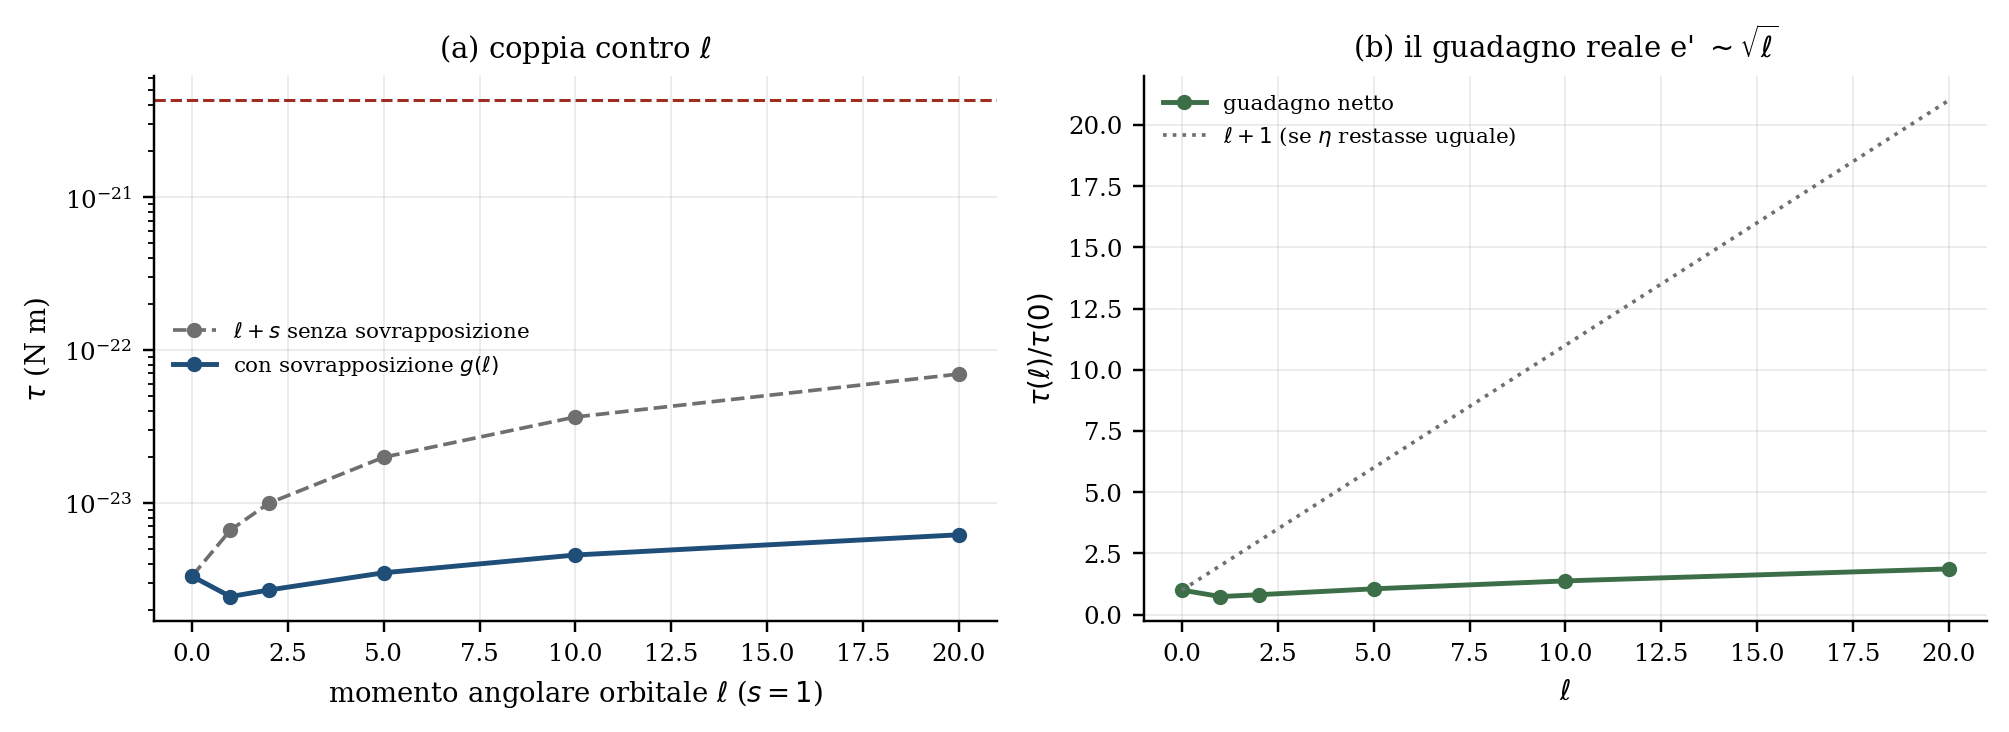
\includegraphics[width=\textwidth]{../figure/fig09_oam.png}
\caption{\textbf{(a)} Torque against $\ell$ with and without the mode overlap.
\textbf{(b)} Net gain: the grey curve is what one would obtain if $\eta$ stayed
constant, the green one is what is obtained.}
\label{fig:oam}
\end{figure}

%=====================================================================
\section{Limits, falsifiability, protocol}
\label{sec:limiti}
%=====================================================================

\subsection{What V6 has not done}
\begin{enumerate}\itemsep2pt
\item \textbf{Full-wave calculation of the whole frame.} The superposition is
incoherent and declared; a DDA/FDTD run can change $\sigma_{\rm pr}$ by a factor 4. It
is the first task, and it conditions the entire torque section.
\item \textbf{Per-shape optics.} Disc, ring and dumbbell have a band, not a value.
Without DDA their $Pe_r$ stays conditional.
\item \textbf{Thermo-mechanical coupling.} Temperature is computed in steady state on
a rigid body; differential expansion between core and frame and the resulting loss of
planarity are not treated.
\item \textbf{Counter-spin dynamics.} The 45/376 ratio is treated as a kinematic
constraint; the dynamics of that constraint are not computed.
\item \textbf{Real fluid.} Newtonian water at \SI{20}{\degreeCelsius}; a biological
medium is viscoelastic.
\end{enumerate}

\subsection{How to refute V6}
\begin{enumerate}\itemsep2pt
\item \textbf{Torque against absorbed power.} Equation \eqref{eq:modello} predicts
$\tau/P_{\rm abs}=1/\omega_{\rm ott}=2.82\times10^{-16}$\,s. If a measurement on a
\SI{40}{nm} copper particle exceeds it, the model is incomplete and the scattering
channel transfers angular momentum coherently.
\item \textbf{Dependence on $\beta$.} Identity \eqref{eq:identita} predicts that $Pe_r$
does not change when going from water to water-glycol while $\omega_{\rm ss}$ scales as
$1/\beta$. If $Pe_r$ changes, the drag model is wrong.
\item \textbf{Thermal threshold in vacuum.} V6 predicts melting at
\SI{0.13}{}--\SI{0.66}{\micro W}. If melting occurs at much higher power, the radiative
balance is incomplete (conduction through the levitation medium) or the area is much
larger than the geometric one.
\end{enumerate}

\subsection{Protocol for the full-wave audit}
\begin{itemize}\itemsep1pt
\item Geometry: exact V5 frame, wires 6.4 / 15 / 9 nm, core \SI{40}{nm}.
\item Material: copper with Drude $\varepsilon(a)$, plus a Cu$_2$O shell of 0, 1, 2 nm.
\item Discretisation: step $\le\lambda/20$ in the metal ($\le\SI{13}{nm}$), with
two-step convergence check.
\item Incidence: four orientations, circular polarization.
\item Output: $\sigma_{\rm ext}$, $\sigma_{\rm abs}$, $g$, $\sigma_{\rm pr}$, and the
comparison with the incoherent sum used here.
\end{itemize}

%=====================================================================
\appendix
\section{The 720$^\circ$ cycle and the 45/376 ratio}
\label{app:su2}
%=====================================================================

This material should be kept, not promoted. Three statements, in decreasing order of
strength.

\textbf{First, solid.} The V5 scene completes exactly 720$^\circ$ on the Spin and
86.1702$^\circ$ on the Counter-spin in 240 frames, with absolute keyframes and no
reduction modulo 360. It is a verifiable fact in the \texttt{.blend} file and in the
code.

\textbf{Second, conventional.} The double cover of $SO(3)$ is a property of $SU(2)$:
$U(\theta)=\exp(-i\theta\sigma_z/2)$ changes sign at $2\pi$ and returns to $+1$ at
$4\pi$. A rotor is a macroscopic classical body and its geometric periodicity is
$2\pi$; the $4\pi$ periodicity is a construction choice of the animation, not a
measurable signature.

\textbf{Third, not to be used.} The ratio $I_2/I_1=45/376$ closes the kinematics, not
the dynamics. V5 achieved closure by adding $3.06\times10^{-20}$\,kg at \SI{42}{nm}
from the centre ($2.9\times10^5$ copper atoms, $1.1$\,\% of the frame mass). V6 does not
use that mass: the point of application falls inside the core and corresponds to no
element of the scene. Above all, nothing guarantees that the optical and dissipative
torques spontaneously produce that ratio. A rational ratio between two angular
velocities guarantees geometric repetition \emph{if} the ratio is maintained;
maintenance requires a mechanical constraint, and a mechanical constraint between two
rotors makes them a single rigid body with a single moment of inertia. The
Counter-spin cannot be at the same time independent (to have a ratio of its own) and
constrained (to keep it).

The ratio 45/376 remains a property of the shape, invariant over nine orders of
magnitude in scale and across the three materials. As such it should be cited, without
the balancing mass and without the quantum aura that V4 attributed to it.

\begin{figure}[H]
\centering
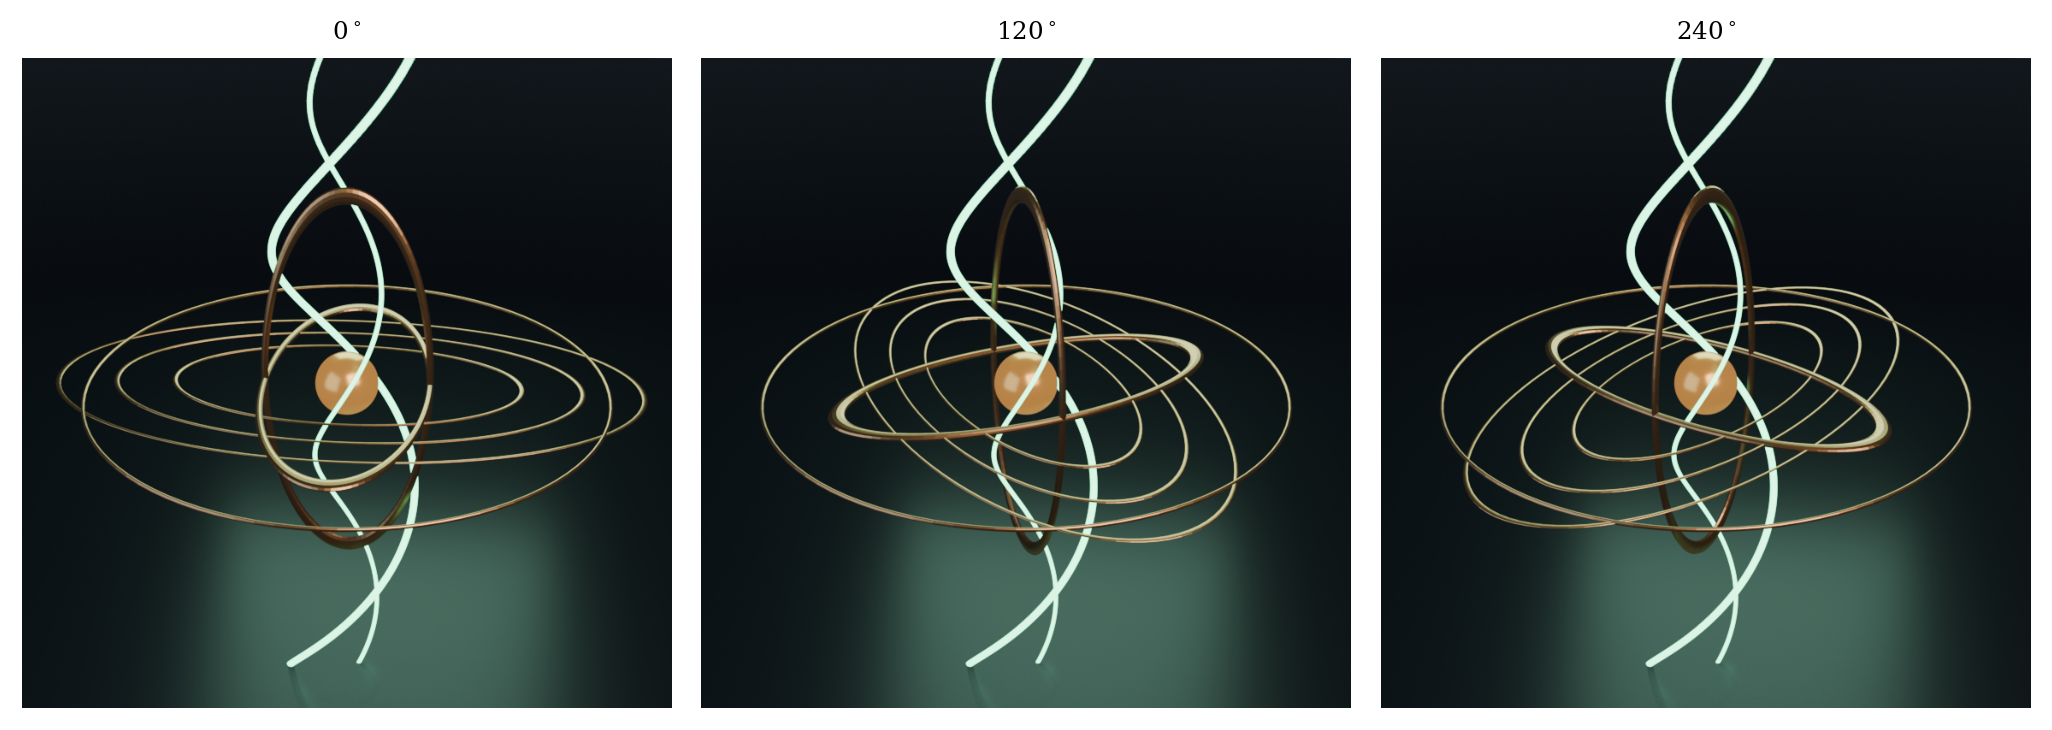
\includegraphics[width=\textwidth]{../figure/fig12_sequenza.png}
\caption{Three orientations of the scene at 0, 120 and 240$^\circ$. The animation is a
check of geometric consistency of the cycle, not a physical simulation.}
\label{fig:sequenza}
\end{figure}

\section{Excluded material and its destination}

Two themes of V5 do not enter V6, and this is not an oversight. The \emph{ark} and the
\emph{blood} --- cosmological metaphors and the reference to a biological medium as a
justification for the design --- belong to a different discourse, and mixing them with
a dimensional analysis weakens both: they belong in a separate text. \emph{Pulsed
operation} remains, but demoted to a thermal lever (\S\ref{sec:termica}): the
mechanical time constant of \SI{1.1}{ns} makes it impossible for pulsing to change the
dynamics.

\section{Code, data and reproducibility}

Every number in the text comes from one of four scripts, none of which contains
hard-coded data.

\begin{center}\small
\begin{tabular}{p{3.4cm}p{9.4cm}}
\toprule
file & function \\
\midrule
\texttt{v6\_nucleo.py} & optics (Mie, cylinder, core-shell), drag, thermal, dynamics;
self-test \\
\texttt{v6\_studi.py} & the nine studies, JSON in \texttt{dati/}, tables in
\texttt{tabelle/} \\
\texttt{v6\_figure.py} & the twelve figures from the computed records \\
\texttt{v6\_blender.py} & the scene and the renders in \texttt{blender/} \\
\bottomrule
\end{tabular}
\end{center}

The self-test checks convergence of the cylindrical series against Rayleigh, the
conservation $Q_{\rm ext}\ge Q_{\rm sca}$, identity \eqref{eq:identita} and the limits
of the coated sphere. Anyone wishing to contest a number must contest one of these
checks: that is the point of a revision.

\section*{Acknowledgements}
\addcontentsline{toc}{section}{Acknowledgements}
This revision stems from an external critique that indicated the residuals, the
five-phase structure, the four-question criterion and, in 6.1, the five material errors
corrected here: wire radii, the number $0.119667646$, the radiating area, the
circularity of the baseline and the single point in the GHz comparison. V6 is an
execution of that programme.

\begin{thebibliography}{9}\small
\bibitem{bh} C.~F. Bohren, D.~R. Huffman, \emph{Absorption and Scattering of Light
by Small Particles}, Wiley, New York, 1983, ch.~4 (spheres), ch.~5 (coated spheres),
ch.~8 (cylinders).
\bibitem{jc} P.~B. Johnson, R.~W. Christy, Optical constants of the noble metals,
\emph{Phys. Rev. B} \textbf{6}, 4370--4379 (1972).
\bibitem{kerker} M.~Kerker, \emph{The Scattering of Light and Other Electromagnetic
Radiation}, Academic Press, New York, 1969, ch.~5 (Maxwell-Garnett).
\bibitem{ll} L.~D. Landau, E.~M. Lifshitz, \emph{Fluid Mechanics}, 2nd ed., Pergamon,
1987, \S\,20: a disk rotating about its axis, $M=(32/3)\mu R^3\Omega$.
\bibitem{cox} R.~G. Cox, The motion of long slender bodies in a viscous fluid,
\emph{J. Fluid Mech.} \textbf{44}, 791--810 (1970).
\bibitem{bat} G.~K. Batchelor, Slender-body theory for particles of arbitrary
cross-section in Stokes flow, \emph{J. Fluid Mech.} \textbf{44}, 419--440 (1970).
\bibitem{nair} R.~R. Nair et al., Fine structure constant defines visual transparency
of graphene, \emph{Science} \textbf{320}, 1308--1310 (2008).
\bibitem{marston} P.~L. Marston, J.~H. Crichton, Radiation torque on a sphere caused by
a circularly-polarized electromagnetic wave, \emph{Phys. Rev. A} \textbf{30},
2508--2516 (1984).
\bibitem{reimann} R.~Reimann et al., GHz rotation of an optically trapped nanoparticle
in vacuum, \emph{Phys. Rev. Lett.} \textbf{121}, 033602 (2018).
\bibitem{ahn} J.~Ahn et al., Ultrasensitive torque detection with an optically
levitated nanorotor, \emph{Nat. Nanotechnol.} \textbf{15}, 89--93 (2020).
\bibitem{v5} F.~Bulla, \emph{Photonic Engine of the Vacuum V5}, preprint, 2026 (source
document for all values cited as ``V5'').
\end{thebibliography}

\end{document}
